\documentclass[a4paper,12pt, openany]{book}


%%% Работа с русским языком
\usepackage{cmap}          % поиск в PDF
\usepackage[T2A]{fontenc}      % кодировка
\usepackage[utf8]{inputenc}    % кодировка исходного текста
%\usepackage{fixint}
\usepackage[russian]{babel}  % локализация и переносы
%\usepackage{pscyr}
\usepackage{mathtools, nccmath}
%\renewcommand{\rmdefault}{cmss}
%%% Дополнительная работа с математикой
\usepackage{amsmath,amsfonts,amssymb,amsthm,mathtools} % AMS
\usepackage{titlesec}
\titleformat{\section}{\filcenter\rmfamily\Large\bfseries}{\thesection.}{0.2em}{}
\titleformat{\subsection}{\filcenter\rmfamily\large\bfseries}{\thesubsection.}{0.2em}{}
\titleformat{\subsubsection}{\filcenter\rmfamily\large\bfseries}{\thesubsubsection.}{0.2em}{}
%% Номера формул
%\mathtoolsset{showonlyrefs=true} % Показывать номера только у тех формул, на которые есть \eqref{} в тексте.
%\usepackage{leqno} % Нумерация формул слева
%\usepackage{rumathgrk1}
%\usepackage{MnSymbol}
%% Перенос знаков в формулах (по Львовскому)
\newcommand{\hm}[1]{#1\nobreak\discretionary{}{\hbox{\ensuremath{#1}}}{}}
%\usepackage{glonti}
%%% Работа с картинками
\usepackage{graphicx}  % Для вставки рисунков
\graphicspath{{images/}}  % папки с картинками
\usepackage{wrapfig} % Обтекание рисунков текстом
\addto\captionsrussian{\def\refname{Список используемой литературы}}
%%% Работа с таблицами
\usepackage{array,tabularx,tabulary} % Дополнительная работа с таблицами
\usepackage{longtable}  % Длинные таблицы
\usepackage{multirow} % Слияние строк в таблице
%%% Теоремы
\theoremstyle{plain} % Это стиль по умолчанию, его можно не переопределять.
\newtheorem{theorem}{Теорема}[section]
\newtheorem{proposition}[theorem]{Утверждение}
\usepackage{subcaption}
\theoremstyle{definition} % "Определение"
\newtheorem{corollary}{Следствие}[theorem]
\newtheorem{problem}{Задача}[section]
\pagestyle{plain}
\theoremstyle{remark} % "Примечание"
\newtheorem*{nonum}{Решение}
%\pagestyle{empty}
%%% Страница
\usepackage{extsizes} % Возможность сделать 14-й шрифт
\usepackage{geometry} % Простой способ задавать поля
\geometry{top=20mm}
%\geometry{bottom=35mm}
\geometry{left=20mm}
\geometry{right=20mm}
\setlength{\parindent}{1.1cm}
%\numberwithin{equation}{section}
\usepackage{setspace} % Интерлиньяж
%\onehalfspacing % Интерлиньяж 1.5
%\doublespacing % Интерлиньяж 2
%\singlespacing % Интерлиньяж 1
\makeatletter
\def\@biblabel#1{#1. }
\makeatother
\usepackage{misccorr}
\usepackage{lastpage} % Узнать, сколько всего страниц в документе.
\usepackage[usenames]{color}
\usepackage{colortbl}
\renewcommand{\baselinestretch}{1.07}
\usepackage{hyperref}
\usepackage[usenames,dvipsnames,svgnames,table]{xcolor}
\hypersetup{        % Гиперссылки
  unicode=true,           % русские буквы в раздела PDF
  pdftitle={Заголовок},   % Заголовок
  pdfauthor={Автор},      % Автор
  pdfsubject={Тема},      % Тема
  pdfcreator={Создатель}, % Создатель
  pdfproducer={Производитель}, % Производитель
  pdfkeywords={keyword1} {key2} {key3}, % Ключевые слова
  colorlinks=true,         % false: ссылки в рамках; true: цветные ссылки
  linkcolor=black,          % внутренние ссылки
  citecolor=blue,        % на библиографию
  filecolor=magenta,      % на файлы
  urlcolor=cyan           % на URL
}
\usepackage{bm}
\newcommand{\dd}{\mathrm{d}}
\numberwithin{equation}{chapter}

\begin{document}

\newpage
\thispagestyle{empty}


% НАЧАЛО ТИТУЛЬНОГО ЛИСТА
\begin{center}
\large{\textsc{ФЕДЕРАЛЬНОЕ ГОСУДАРСТВЕННОЕ БЮДЖЕТНОЕ ОБРАЗОВАТЕЛЬНОЕ
УЧРЕЖДЕНИЕ ВЫСШЕГО ОБРАЗОВАНИЯ}
}\\
\large{\textsc{МОСКОВСКИЙ ГОСУДАРСТВЕННЫЙ УНИВЕРСИТЕТ имени М.В. ЛОМОНОСОВА}
} \\
 \vspace{0.4cm}
\large{\textsc{МЕХАНИКО- МАТЕМАТИЧЕСКИЙ ФАКУЛЬТЕТ}}\\
\vspace{0.4cm}
\large{\textsc{КАФЕДРА ПРИКЛАДНОЙ МЕХАНИКИ И УПРАВЛЕНИЯ}}\\
\hfill \break

\hfill \break
\large{\textbf{ВЫПУСКНАЯ КВАЛИФИКАЦИОННАЯ РАБОТА}\\
(ДИПЛОМНАЯ РАБОТА) \\ МАГИСТРА \\
\hfill \break \textsc{\textbf{ВОССТАНОВЛЕНИЕ ЧЕЛОВЕКОМ ИСХОДНОЙ ПОЗЫ ПОСЛЕ ТОЛЧКА} \\
\textbf{REVERSION OF INITIAL POSTURE BY A PERSON AFTER A PUSH}
}}
\end{center}
 
\vspace{1.5cm}
\begin{flushright}
\large{
Выполнил: студент группы М - 2 \\ Романов Андрей Владимирович} \\ \vspace{0.68cm}  \underline{\hspace{6.5cm}} \\ 
 (подпись студента)

\end{flushright}
 
\begin{flushright}
\large{
Научный руководитель: \\ к.ф.-м.н., доцент Кручинин Павел Анатольевич} \\ \vspace{0.68cm}
 \underline{\hspace{6.5cm}} \\
 (подпись научного руководителя)
\end{flushright}
\vspace{0.7cm}
\begin{center} \large{Москва  2023 год} \end{center}



\thispagestyle{empty} % выключаем отображение номера для этой страницы
 \normalsize{
% КОНЕЦ ТИТУЛЬНОГО ЛИСТА
\newpage

\tableofcontents

\newpage

\addcontentsline{toc}{chapter}{Введение}

\chapter*{Введение}
В литературе встречается решение задач оптимального быстродействия для моделей движения человека \cite{pandy,humanMovements}. Исследование таких задач может помочь объяснить некоторые особенности результатов, наблюдаемых при обследованиях.
Проба со ступенчатым воздействием является одной из стандартных проб
при стабилометрических исследованиях \cite{AdaptFizkult,stabilographTest}. При проведении этой пробы
обследуемый стоит на платформе стабилоанализатора перед экраном, на
котором изображена мишень и отображается движение центра давления
человека, после толчка в спину, определяемое по показаниям стабилоанализатора.

В ходе теста производят толкающее воздействие на человека с помощью груза, помещенного на подвижном отвесе \cite{pusher}. В результате внешнего
воздействия тело человека наклоняется вперед и при не очень сильном толчке
он не теряет равновесие и не падает, а возвращается в исходное
положение за счет изменения угла в голеностопном суставе. Изменение
остальных суставных углов может оказаться тоже не столь значительным.
Родственные задачи уже решались в работах \cite{PAKrychinin,kasatkin}.
Схематическое изображение эксперимента представлено на рисунке \ref{fig:pusher}.
\begin{figure}[h!]
    \centering
    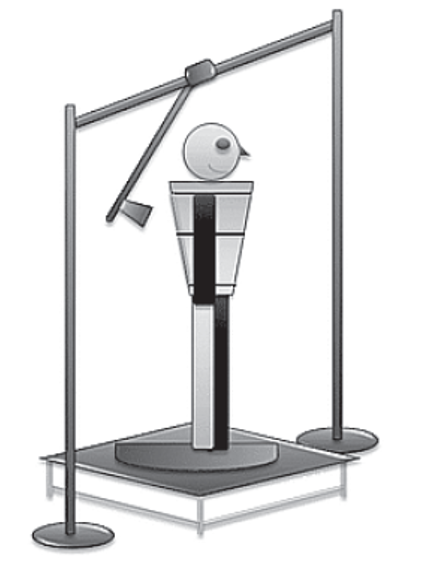
\includegraphics[width=0.35\linewidth]{human.png}
    \caption{Cхематическое изображение толкателя и
        положения испытуемого на стабилоплатформе}
    \label{fig:pusher}
\end{figure}

Исходные данные об отклонении сагиттальной коордианты при различных по силе толчках, предоставлены сотрудниками ИМБП РАН (см. рисунок \ref{fig:pushes})
\begin{figure}[h!]
    \centering
    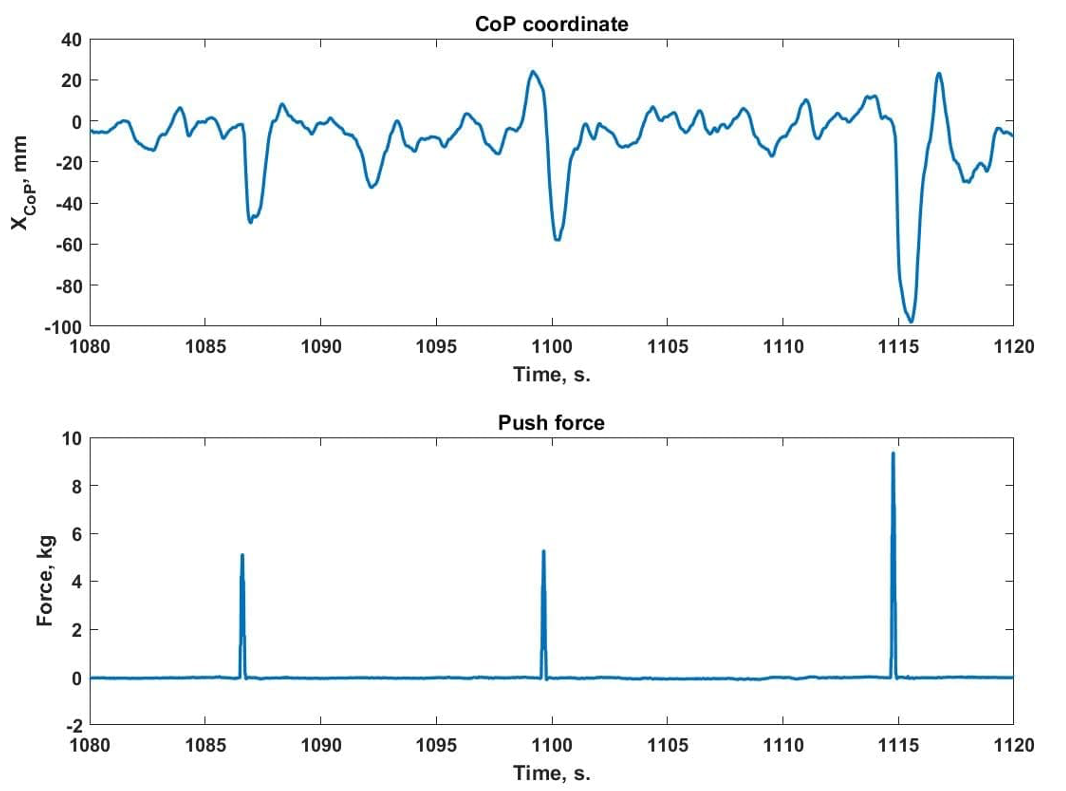
\includegraphics[width=0.9\linewidth]{Pushes.png}
    \caption{Отклонение сагиттальной координаты при различных по силе толчках}
    \label{fig:pushes}
\end{figure}

В курсовой работе предполагается рассмотреть возможные
алгоритмы управления изменением позы человека, основанные на решении задачи
оптимального быстродействия, которые можно было бы использовать для
возвращения человека в исходную вертикальную позу. В качестве математической модели
используется модель «перевернутого маятника»\cite{PAKrychinin,kasatkin,gurfincel}. В дальнейшем
такое решение предполагается использовать для оценки эффективности управления человеком
при возвращении в вертикальную позу, путем сравнения
времени реального процесса с полученным эталонным решением оптимальной задачи.


\textbf{Целью работы} является разработка алгоритма управления изменением позы человека, основанного на решении задачи оптимального быстродействия,
который можно было бы использовать для возвращения в исходную вертикальную позу

\textbf{Задачи работы: }
\begin{itemize} 
    \item Описание математической модели
    \item Постановка задачи быстродействия, используя принцип максимума Понтрягина
    \item Поиск решения задачи быстродействия
    \item Определение начального состояния системы, в момент завершения толчка
    \item Решение задачи быстродействия с вычисленными начальными условиям
    \item Сравнение реального и оптимального времени возвращения в исходную позу
    \item Сравнение реальной и оптимальной траектории возварщения в исходную позу
    \item Интерпретация полученных результатов
\end{itemize} 

\textbf{Методы исследования.} Для решения оптимальных задач используется принцип максимума Понтрягина, качественное исследование полученных дифференциальных уравнений проводится с помощью метода фазовой плоскости. Краевые задачи, полученные из принципа максимума Понтрягина, решаются с помощью численных методов решения задач оптимального управления (метод стрельбы, метод дихотомии и Ньютона). 

\textbf{Объем и структура работы.} Работа состоит из введения, трех глав и заключения. Полный объем работы составляет 61 страницу, включая 69 рисунков и 1 таблицу. Список литературы содержит 17 наименований. 

\newpage

\chapter{Оптимальное уклонение цели от преследователя, использующего метод пропорционального наведения}

\section{Постановка задачи}

Пусть в горизонтальной плоскости (рис. \ref{picture1}) движутся две материальные точки:  преследователь $P$ и цель $E$, $\theta$ -- угол между линией $PE$ и осью $Ox$, $\beta$ -- угол между линией $PE$ и направлением вектора скорости преследователя $v_P$, $\alpha$ -- угол между линией $PE$ и направлением вектора скорости цели $v_E$. 





Уравнения движения материальных точек в безразмерном виде

\begin{equation}\label{2.1}
\left\{ \begin{aligned}
	&\dot r = \cos \alpha  - b\cos \beta , \\ 
	&\dot \beta  = \dfrac{{b\sin \beta  - \sin \alpha }}{{rc}}, \\ 
	&\dot \alpha  = \dfrac{{b\sin \beta  - \sin \alpha }}{r} + u, \\ 
\end{aligned} \right.
\end{equation} 
где $b = v_P/v_E, \, c = -\mfrac{1}{k-1}$, $k>1$ -- коэффициент в $\dot{\beta} = k\dot{\theta}$ (метод пропорционального наведения), $u$ -- управление, $\left|u\right|<\infty$.  
\newpage
В работе рассматриваются случаи, когда $0<b<1$ и $b\geqslant 1$. 
Начальные условия имеют вид
\begin{equation}\label{2.2}
	r(0) = r_0, \quad \beta(0) = \beta_0, \quad \alpha(0) = \alpha_0.
\end{equation}
Считая теперь, что $\alpha(0)$ свободно, можно провести редукцию системы \eqref{2.1}. Вместо управления $u$ выбирается $\alpha$ и рассматривается система
\begin{equation}\label{2.3}
	\left\{ \begin{aligned}
		&\dot r = \cos \alpha  - b\cos \beta , \\ 
		&\dot \beta  = \dfrac{{b\sin \beta  - \sin \alpha }}{{rc}}, \\ 
		\end{aligned} \right.
\end{equation} 
Начальные условия в этом случае имеют вид:
\begin{equation}\label{2.4}
	r(0) = r_0, \quad \beta(0) = \beta_0.
\end{equation}

Время окончания процесса $T$ фиксировано. Цель управления -- максимизация конечного расстояния между объектами:
\begin{equation}\label{2.5}
\mathcal{J} = -r\left( T \right) \to \mathop {\min }\limits_{u\left(  \cdot  \right) \in U} 
\end{equation}

 \section{Сведение к краевой задаче}
 

Введем в рассмотрение функцию Понтрягина $H$ \cite{Optimal}, которая представляется в виде 
\begin{equation}\label{2.6}
H(\bm{\psi},\bm {x},u) = \bm{\psi}^\top \bm{f}, 
\end{equation}
где $
\bm{\psi}  = \left( {\psi _1 , \ldots ,\psi _n } \right)^\top
$ -- сопряженные переменные, $
\bm{f}  = \left( {f _1 , \ldots ,f _n } \right)
$ -- правые части дифференциальных уравнений, относящихся к задаче, $\bm{ x} = (x_1,\ldots, x_n)^\top$ -- фазовые переменные. 

В данной задаче $
\bm{\psi}  = \left( {\psi _r ,\psi _\beta  } \right)^\top
$, $\bm{y} = (r,\beta)^\top$, $
\bm{f}  = \left( {f _1 ,f _2 } \right)^\top
$, где $$
f _1   = \cos \alpha  - b\cos \beta, \quad f_2  = \frac{1}{{rc}}\left( {b\sin \beta  - \sin \alpha } \right).
$$
Тогда функция Понтрягина \eqref{2.6} примет вид
\begin{equation}\label{2.7}
H = \psi _r \left( {\cos \alpha  - b\cos \beta } \right) + \frac{{\psi _\beta  }}{{rc}}\left( {b\sin \beta  - \sin \alpha } \right),
\end{equation}
и равна константе $C$ на оптимальной траектории. 

Сопряженная система
\begin{equation}\label{2.8}
\bm{\dot \psi}  =  - \frac{{\partial H}}
{{\partial \bm{x}}},
\end{equation}
После подстановки \eqref{2.7} в уравнения \eqref{2.8} получим:
\begin{equation} \label{2.9}
\left\{ {\begin{aligned}
   & \dot \psi _r  =  - \frac{{\partial H}}{{\partial r}} = \frac{{\psi _\beta  }}{{r^2 c}}\left( {b\sin \beta  - \sin \alpha } \right), \hfill  \\
  & \dot \psi _\beta   =  - \frac{{\partial H}}{{\partial \beta }} =  - \psi _r b\sin \beta  - \frac{{\psi _\beta  }}{{rc}}b\cos \beta . \hfill  \\
\end{aligned}} \right.
\end{equation}

Условия трансверсальности \cite{Letov}:
\[
\left\{ {\delta \mathcal{J} - H\delta t + \sum\limits_{i = 1}^n {\psi _i \delta x_i } } \right\}_{t = 0}^{t = T}  = 0,
\]
где $\mathcal{J} = -r(T), \,\psi_1 = \psi_r, \, \psi_2 = \psi_{\beta}, \, x_1 = r, \, x_2 = \beta$. Откуда получаем:
\begin{equation}\label{2.10}
\psi_r(T) = 1, \quad \psi_{\beta}(T) = 0.
\end{equation}

Необходимое условие максимума функции $H$ по управлению $\alpha$ :
\begin{equation} \label{2.11}
\frac{{\partial H}}{{\partial \alpha }} =  - \psi _r \sin \alpha  - \frac{{\psi _\beta  }}{{rc}}\cos \alpha  = 0 \Longleftrightarrow \psi _r \sin \alpha  \cdot rc =  - \psi _\beta  \cos \alpha .
	\end{equation}	
Отсюда следует, что функции $\psi_r, \, \psi_\beta$ и $\alpha$ имеют один и тот же класс гладкости. Первоначально предполагалось, что $\alpha$ -- кусочно-непрерывная функция. Поскольку сопряженные переменные удовлетворяют дифференциальным уравнениям \eqref{2.9}, то они являются гладкими функциями, а значит и $\alpha$ также гладкая функция. 

Таким образом, уравнения \eqref{2.3}, \eqref{2.9}, \eqref{2.11} образуют замкнутую систему дифференциальных уравнений относительно $r, \, \beta, \, \psi_r, \, \psi_\beta$, поскольку управление $\alpha$ можно выразить из условия \eqref{2.11} через $\psi_r$, $\psi_\beta$.  

Проанализируем условие оптимальности \eqref{2.11}. При $t = T$ получим:  
$$\psi_r(T)\sin\alpha(T) \cdot r(T) c = -\psi_\beta(T)\cos\alpha(T).$$
Поскольку $\psi_\beta(T) = 0$, то $\psi_r(T)\sin\alpha(T) \cdot r(T) c = 0$. Считая, что в конечный момент времени $r(T) \neq 0$, получим $\psi_r(T)\sin\alpha(T) = 0$, откуда $\psi_r(T) = 0$ или $\sin\alpha(T) = 0$. 

$\psi_r(T) \neq 0$ в силу \eqref{2.10}, тогда $\sin\alpha(T) = 0$, откуда $\cos\alpha(T) = \pm 1$. Чтобы определиться со знаком, найдем вторую производную функции Понтрягина 
\[
\frac{{\partial ^2 H}}{{\partial \alpha ^2 }} =  - \psi _r \cos \alpha  + \frac{{\psi _\beta  }}{{rc}}\sin \alpha .
\]
При $t = T$ 
\[
\left. {\frac{{\partial ^2 H}}{{\partial \alpha ^2 }}} \right|_{t = T}  =  - \psi _r \left( T \right)\cos \alpha \left( T \right) < 0 \Longleftrightarrow \cos \alpha \left( T \right) > 0.
\]
Поэтому $\cos\alpha(T) = 1$ и $\alpha(T) = 0$.

Получим уравнение для $\alpha(t)$. Для этого продифференцируем левую и правую часть условия оптимальности \eqref{2.11}
\begin{equation}\label{2.12}
\dot \psi _r \,\tg\alpha  + \psi _r \frac{{\dot \alpha }}{{\cos ^2 \alpha }} = \frac{{\psi _\beta  \,\dot r}}{{r^2 c}} - \frac{{\dot \psi _\beta  }}{{rc}}.
\end{equation}
Производные сопряженных функций можно выразить из \eqref{2.9}, поэтому условие \eqref{2.12} можно рассматривать как уравнение относительно $\dot{\alpha}$. Из \eqref{2.12} выражаем $\dot{\alpha}$ и проводим преобразования с учетом условия \eqref{2.11}:
\begin{equation}\label{2.13}
\dot \alpha  = \frac{{\dot r\psi _\beta  }}{{\psi _r }} \cdot \frac{1}{{r^2 c}}\cos ^2 \alpha  - \frac{{\dot \psi _\beta  }}{{\psi _r }} \cdot \frac{1}{{rc}}\cos ^2 \alpha  - \frac{{\dot \psi _r }}{{\psi _r }}\sin \alpha \cos \alpha.
\end{equation}
Отдельно преобразуем каждое слагаемое в \eqref{2.13}:
\begin{multline*}
\frac{{\dot r\psi _\beta  }}{{\psi _r }} \cdot \frac{1}{{r^2 c}}\cos ^2 \alpha  =  - \frac{{rc}}{{r^2 c}}\tg\alpha \cos ^2 \alpha \cdot \dot r =  - \frac{{\sin \alpha }}{{\cos \alpha }} \cdot \frac{{\dot r}}{r}\cos ^2 \alpha  =  \\
 =  - \frac{{\dot r}}{r}\sin \alpha \cos \alpha  = \frac{1}{r}\sin \alpha \cos \alpha \left( {b\cos \beta  - \cos \alpha } \right), 
\end{multline*}
\begin{multline*}
 - \frac{{\dot \psi _\beta  }}{{\psi _r }} \cdot \frac{1}{{rc}}\cos ^2 \alpha  = \frac{1}{{\psi _r }} \cdot \frac{1}{{rc}}\cos ^2 \alpha \left( {\psi _r b\sin \beta  + \frac{{\psi _\beta  }}{{rc}}b\cos \beta } \right) =  \\
 = \frac{1}{{rc}}b\sin \beta \cos ^2 \alpha  + \frac{{\psi _\beta  }}{{\psi _r }} \cdot \frac{b}{{r^2 c^2 }}\cos ^2 \alpha \cos \beta  = \frac{1}{{rc}}b\sin \beta \cos ^2 \alpha  -  \\
 - \frac{{b\tg\alpha }}{{rc}}\cos ^2 \alpha \cos \beta  = \frac{b}{{rc}}\cos \alpha \sin \left( {\beta  - \alpha } \right),
\end{multline*}
\begin{multline*}
 - \frac{{\dot \psi _r }}{{\psi _r }}\sin \alpha \cos \alpha  =  - \frac{{\psi _\beta  }}{{\psi _r }} \cdot \frac{1}{{r^2 c}}\sin \alpha \cos \alpha \left( {b\sin \beta  - \sin \alpha } \right) = \\
 =  - \frac{1}{{r^2 c}}\frac{{\psi _\beta  }}{{\psi _r }}\sin \alpha \cos \alpha \left( {b\sin \beta  - \sin \alpha } \right) = \frac{1}{r}\sin ^2 \alpha \left( {b\sin \beta  - \sin \alpha } \right). 
\end{multline*}
Подставляем полученные выражения в \eqref{2.13}:
\begin{equation*}
\dot \alpha  = \frac{1}{r}\sin \alpha \cos \alpha \left( {b\cos \beta  - \cos \alpha } \right) + \frac{b}{{rc}}
\cos \alpha \sin \left( {\beta  - \alpha } \right) - \frac{1}{r}\sin ^2 \alpha \left( {\sin \alpha  - b\sin \beta } \right).
\end{equation*}
Окончательно после всех преобразований получаем уравнение на $\alpha$:
\begin{equation}\label{2.14}
\dot \alpha  = \frac{1}{r}\sin \alpha \left( {b\cos \left( {\alpha  - \beta } \right) - 1} \right) + \frac{b}{{rc}}\cos \alpha \sin \left( {\beta  - \alpha } \right)
\end{equation}
Объединяя уравнения \eqref{2.3} и \eqref{2.14}, получим систему дифференциальных уравнений относительно неизвестных $r(t), \, \beta(t), \, \alpha(t)$: 
\begin{equation}\label{2.15}
\left\{ {\begin{aligned}
   &\dot r = \cos \alpha  - b\cos \beta , \hfill  \\
   &\dot \beta  = \frac{{b\sin \beta  - \sin \alpha }}{{rc}}, \hfill  \\
   &\dot \alpha  = \frac{1}{r}\sin \alpha \left( {b\cos \left( {\alpha  - \beta } \right) - 1} \right) + \frac{b}{{rc}}\cos \alpha \sin \left( {\beta  - \alpha } \right). \hfill  \\
\end{aligned}} \right.
\end{equation}
Краевые условия
\begin{equation}\label{2.16}
r\left( 0 \right) = r_0 ,\,\,\beta  \left( 0 \right) = \beta _0 ,\,\,\alpha \left( T \right) = 0.
\end{equation}
\newpage
Задача оптимального управления \eqref{2.3}, \eqref{2.4}, \eqref{2.5} сведена к краевой задаче для системы нелинейных дифференциальных уравнений \eqref{2.15}, \eqref{2.16}. Если решение задачи найдено, т.е. известны функции $r(t)$, $\beta(t)$, $\alpha(t)$, то управление $u(t)$ можно найти из \eqref{2.1} с учетом \eqref{2.14}
\begin{equation}\label{2.17}
u\left( t \right) = \frac{1}{r}\sin \alpha \left( {b\cos \left( {\alpha  - \beta } \right) - 1} \right) + \frac{b}{{rc}}\cos \alpha \sin \left( {\beta  - \alpha } \right) - \frac{{b\sin \beta  - \sin \alpha }}{r}.
\end{equation}


\section{Качественное исследование полученной системы}
\subsection{Нахождение положений равновесия}
\subsubsection*{Случай $b \neq 1$}

Рассмотрим систему \eqref{2.15}. Прежде чем переходить к численному решению задачи \eqref{2.15} -- \eqref{2.16}, проведем качественное исследование. Заметим, что второе и третье уравнения системы \eqref{2.15} содержат неизвестную функцию $r$ в знаменателе, поэтому можно провести анализ этих двух уравнений относительно функций $\alpha, \, \beta$.
\begin{equation}\label{2.18}
\left\{ {\begin{aligned}
   &\dot \alpha  = \frac{1}{r}\sin \alpha \left( {b\cos \left( {\alpha  - \beta } \right) - 1} \right) + \frac{b}{{rc}}\cos \alpha \sin \left( {\beta  - \alpha } \right), \hfill  \\
   &\dot \beta  = \frac{{b\sin \beta  - \sin \alpha }}{{rc}}. \hfill  \\
\end{aligned}} \right.
\end{equation}
Для начала найдем положения равновесия, т.е. когда $\dot{\alpha} = 0, \, \dot{\beta} = 0$. 
\begin{equation}\label{2.19}
\left\{ {\begin{aligned}
   &b\sin \beta  - \sin \alpha  = 0, \hfill  \\
   &c\sin \alpha \left( {b\cos \left( {\alpha  - \beta } \right) - 1} \right) + b\cos \alpha \sin \left( {\beta  - \alpha } \right) = 0. \hfill  \\
\end{aligned}} \right.
\end{equation}
Преобразуем второе уравнение \eqref{2.19} с учетом первого
\[
bc\sin \beta \left( {b\cos \alpha \cos \beta  + \sin ^2 \alpha  - 1} \right) + b\cos \alpha \left( {\sin \beta \cos \alpha  - \sin \alpha \cos \beta } \right) = 0 \Longleftrightarrow 
\]
\[
 \Longleftrightarrow bc\sin \beta \left( {b\cos \alpha \cos \beta  + \sin ^2 \alpha  - 1} \right) + b\cos \alpha \left( {\sin \beta \cos \alpha  - b\sin \beta \cos \beta } \right) = 0 \Longleftrightarrow 
\]
\[
 \Longleftrightarrow c\sin \beta \left( {b\cos \alpha \cos \beta  + \sin ^2 \alpha  - 1} \right) + \sin \beta \cos \alpha \left( {\cos \alpha  - b\cos \beta } \right) = 0 \Longleftrightarrow 
\]
\[
 \Longleftrightarrow \sin \beta \left[ {c\left( {b\cos \alpha \cos \beta  + \sin ^2 \alpha  - 1} \right) + \cos \alpha \left( {\cos \alpha  - b\cos \beta } \right)} \right] = 0 \Longleftrightarrow 
\]
\[
 \Longleftrightarrow \left[ {\begin{aligned}
   &\sin \beta  = 0, \hfill  \\
   &c\left( {b\cos \alpha \cos \beta  + \sin ^2 \alpha  - 1} \right) + \cos \alpha \left( {\cos \alpha  - b\cos \beta } \right) = 0. \hfill  \\
\end{aligned}} \right.
\]
Из первого уравнения $\sin\beta = 0$, тогда $\sin\alpha = 0$. Если считать $r$ как параметр, то фазовым пространством системы \eqref{2.18} является тор. Поэтому рассмотрим развертку тора на плоскость и ограничимся квадратом $[-\pi,\pi]\times[-\pi,\pi]$. В этом квадрате следующие положения равновесия 
\begin{equation}\label{2.20}
\left( { - \pi ,\pi } \right),\left( { - \pi , - \pi } \right),\left( {\pi , - \pi } \right),\left( {\pi ,\pi } \right),\left( { - \pi ,0} \right),\left( {\pi ,0} \right),\\\left( {0, - \pi } \right),\left( {0,\pi } \right),\left( {0,0} \right).
\end{equation}
Рассмотрим второе уравнение совокупности 
\[
c\left( {b\cos \alpha \cos \beta  + \sin ^2 \alpha  - 1} \right) + \cos \alpha \left( {\cos \alpha  - b\cos \beta } \right) = 0 \Longleftrightarrow 
\]
\[
 \Longleftrightarrow c\left( {b\cos \alpha \cos \beta  - \cos ^2 \alpha } \right) + \cos \alpha \left( {\cos \alpha  - b\cos \beta } \right) = 0 \Longleftrightarrow 
\]
\[
 \Longleftrightarrow c\cos \alpha \left( {b\cos \beta  - \cos \alpha } \right) - \cos \alpha \left( {b\cos \beta  - \cos \alpha } \right) = 0 \Longleftrightarrow 
\]
\[
 \Longleftrightarrow \cos \alpha \left( {b\cos \beta  - \cos \alpha } \right)\left( {c - 1} \right) = 0 \Longleftrightarrow \left[ {\begin{aligned}
   &\cos \alpha  = 0, \hfill  \\
   &b\cos \beta  = \cos \alpha . \hfill  \\
\end{aligned}} \right.
\]
Если $b\cos\beta = \cos\alpha$, то вместе с уравнением $b\sin\beta = \sin\alpha$ получим $\sin^2\alpha + \cos^2\alpha = b^2$, откуда $b = 1$. Если $\cos\alpha = 0$, то $\alpha = \pm\pi/2$. Тогда из первого уравнения \eqref{2.19}  $\sin\beta = 1/b \sin\alpha$. 

При $\alpha = -\pi/2$ получим $\sin\beta = -1/b$ . Если $b\in(0,1)$, то уравнение не имеет решений. Если $b>1$, то $
\beta  =  - \arcsin \left( {1/b} \right),\,\,\beta  =  - \pi  + \arcsin \left( {1/b} \right).
$

При $\alpha = \pi/2$ получим $\sin\beta = 1/b$. Если $b\in(0,1)$, то уравнение не имеет решений. Если $b>1$, то $
\beta  = \arcsin \left( {1/b} \right),\,\,\beta  = \pi  - \arcsin \left( {1/b} \right)
$. Таким образом, получим следующие положения равновесия системы (при $b>1$):
\begin{equation}\label{2.21}
\left( {\mfrac{\pi }{2},\,\arcsin \mfrac{1}{b}} \right),\,\left( {\mfrac{\pi }{2},\,\,\pi  - \arcsin \mfrac{1}{b}} \right),\,\left( { - \mfrac{\pi }{2}, - \arcsin \mfrac{1}{b}} \right),\,\left( { - \mfrac{\pi }{2}, - \pi  + \arcsin \mfrac{1}{b}} \right).
\end{equation}

При $b>1$ имеем 13 положений равновесия \eqref{2.20}, \eqref{2.21}, при $b\in(0,1)$ -- 9 положений равновесия \eqref{2.20}. 

\subsubsection*{Случай $b = 1$}


Отдельно рассмотрим случай, когда $b=1$, т.е. скорости преследователя и цели одинаковые. Тогда система \eqref{2.19} примет вид
\begin{equation}\label{2.22}
\left\{ {\begin{aligned}
   & \sin \beta  - \sin \alpha  = 0, \hfill  \\
   & c\sin \alpha \left( {\cos \left( {\alpha  - \beta } \right) - 1} \right) + \cos \alpha \sin \left( {\beta  - \alpha } \right) = 0. \hfill  \\
\end{aligned}} \right.
\end{equation}
Проводя аналогичные преобразования, описанные выше, приходим к системе
\begin{equation}\label{2.23}
\left\{ {\begin{aligned}
   &\sin \beta  - \sin \alpha  = 0, \hfill  \\
   &\left( {c - 1} \right)\left( {\cos \beta  - \cos \alpha } \right)\sin \alpha \cos \alpha  = 0. \hfill  \\
\end{aligned}} \right. \Longleftrightarrow \left\{ {\begin{aligned}
   \sin \beta  = \sin \alpha , \hfill  \\
   {\left[ {\begin{aligned}
   &\cos \beta  = \cos \alpha , \hfill  \\
   &\sin \alpha  = 0, \hfill  \\
   &\cos \alpha  = 0. \hfill  \\
\end{aligned}} \right.} \hfill  \\
\end{aligned}} \right.
\end{equation}

1) Пусть $\cos\beta = \cos\alpha$. 
$$
\sin \alpha  = \sin \beta  \Longleftrightarrow 2\sin \frac{{\beta  - \alpha }}{2}\cos \frac{{\beta  + \alpha }}{2} = 0 \Longleftrightarrow \left[ {\begin{aligned}
   &\beta  - \alpha  = 2\pi k, \hfill  \\
   &\beta  + \alpha  = \pi  + 2\pi k,\,k \in \mathbb{Z}. \hfill  \\
\end{aligned}} \right.
$$
Поскольку $\alpha,\beta\in[-\pi,\pi]$, то $\beta - \alpha = -2\pi,0,2\pi$, а $\beta+\alpha = -\pi,\pi$. Нетрудно убедиться, что при $\beta - \alpha = -2\pi,0,2\pi$ уравнение $\cos\beta = \cos\alpha$ будет обращаться в тождество. При $\beta + \alpha = -\pi$ получим $\cos\alpha = 0$, откуда $\alpha = \pm\tfrac{\pi}{2}$. При $\alpha = \tfrac{\pi}{2} \Longrightarrow  \beta = -\tfrac{3\pi}{2} \notin [-\pi,\pi]$, при $\alpha = -\tfrac{\pi}{2} \Longrightarrow \beta = -\tfrac{\pi}{2} \in [-\pi,\pi]$.  При $\beta + \alpha = \pi$ получим $\cos\alpha = 0$, откуда $\alpha = \pm\tfrac{\pi}{2}$. При $\alpha = \tfrac{\pi}{2} \Longrightarrow  \beta = \tfrac{\pi}{2} \in [-\pi,\pi]$, при $\alpha = -\tfrac{\pi}{2} \Longrightarrow \beta = \tfrac{3\pi}{2} \notin [-\pi,\pi]$. 

Получим следующие положения равновесия

\begin{equation}\label{2.24}
\left( { - \mfrac{\pi }{2}, - \mfrac{\pi }{2}} \right),\,\,\left( {\mfrac{\pi }{2},\,\mfrac{\pi }{2}} \right).
\end{equation}

2) Пусть $\sin\alpha = 0 \Longrightarrow \alpha = -\pi,0,\pi \Longrightarrow \sin\beta = 0 \Longrightarrow \beta = -\pi,0,\pi$. Получим следующие положения равновесия
\begin{equation}\label{2.25}
\left( { - \pi ,\pi } \right),\left( { - \pi , - \pi } \right),\left( {\pi , - \pi } \right),\left( {\pi ,\pi } \right),\left( { - \pi ,0} \right),\left( {\pi ,0} \right),\\\left( {0, - \pi } \right),\left( {0,\pi } \right),\left( {0,0} \right).
\end{equation}

3) Пусть $\cos\alpha  = 0 \Longrightarrow \alpha = \pm\tfrac{\pi}{2} \Longrightarrow \sin\beta = \pm 1 \Longrightarrow \beta = \pm\tfrac{\pi}{2}$. Получим следующие положения равновесия (с учетом \eqref{2.24})
\begin{equation}\label{2.26}
\left( { - \mfrac{\pi }{2}, - \mfrac{\pi }{2}} \right),\,\,\left( {\mfrac{\pi }{2},\,\mfrac{\pi }{2}} \right),\left( { - \mfrac{\pi }{2},\mfrac{\pi }{2}} \right),\,\left( {\mfrac{\pi }{2}, - \mfrac{\pi }{2}} \right).
\end{equation}

В итоге при $b=1$ имеем 13 положений равновесия \eqref{2.25}, \eqref{2.26}. 

\subsection{Линеаризация системы в окрестности положений равновесия}

Система \eqref{2.14} представляет собой автономную систему дифференциальных уравнений. Проведем ее линеаризацию системы в окрестности положений равновесия \eqref{2.20} и \eqref{2.21}. Систему \eqref{2.18} можно записать в виде
\begin{equation} \label{2.27}
\dot {\bm{x}} = \bm{f}\left( {\bm{x}} \right),
\end{equation}
где $\bm{x} = \left(\alpha,\beta\right)^\top,\,\,\bm{f} \left( {\bm{x}} \right) = \left(F(\alpha,\beta),\,G(\alpha,\beta) \right)^\top$, $F$ и $G$ -- правые части уравнений в системе \eqref{2.14}.

С точностью до слагаемых второго порядка малости получим линейную систему вида
\begin{equation}\label{2.28}
\dot{\bm{x}} = \mathcal{A}\bm{x},\,\,
\end{equation}
где  $\mathcal A$ -- матрица Якоби \cite{Filippov} первых частных производных функций $F$ и $G$, вычисленная в положении равновесия $\bm{x}= \bm{x_0}$:
\begin{equation}\label{2.29}
\mathcal{A} = \left. {\left( {\begin{array}{*{20}c}
   {\mfrac{{\partial F}}
{{\partial \alpha }}} & {\mfrac{{\partial F}}
{{\partial \beta }}} \hfill  \\  [5pt]
   {\mfrac{{\partial G}}
{{\partial \alpha }}} & {\mfrac{{\partial G}}
{{\partial \beta }}}  \\

 \end{array} } \right)} \right|_{\bm{x} = \bm{x_0} } .
\end{equation}
Вычислим их отдельно
\begin{equation}\label{2.30}
\begin{gathered}
\mfrac{{\partial F}}
{{\partial \alpha }}  = \frac{1}
{r}\cos \alpha \left( {b\cos \left( {\alpha  - \beta } \right) - 1} \right) - \frac{1}
{r}\sin \alpha \sin \left( {\alpha  - \beta } \right) - \frac{b}
{{rc}}\cos \left( {2\alpha  - \beta } \right). \hfill \\
\mfrac{{\partial F}}
{{\partial \beta }}  = \frac{b}{r}\sin \alpha \sin \left( {\alpha  - \beta } \right) + \frac{b}{{rc}}\cos \alpha \cos \left( {\beta  - \alpha } \right),
\mfrac{{\partial G}}
{{\partial \alpha }}  =  - \frac{{\cos \alpha }}{{rc}},\,\,\mfrac{{\partial G}}
{{\partial \beta }} = \frac{{b\cos \beta }}{{rc}}.
\end{gathered}
\end{equation}
При подстановке полученных положений равновесий \eqref{2.20} и \eqref{2.21} в \eqref{2.29} будем получать линейную систему дифференциальных уравнений \eqref{2.28}. Их характер определяется путем нахождения корней характеристического уравнения
\begin{equation}\label{2.31}
\det \left( {{\mathcal{A}} - \lambda\,\mathcal{I}} \right) = 0 \Longleftrightarrow \left| {\begin{array}{*{20}c}
   {\mfrac{{\partial F}}
{{\partial \alpha }}  - \lambda } & {\mfrac{{\partial F}}
{{\partial \beta }} }  \hfill  \\  [5pt]
   {\mfrac{{\partial G}}
{{\partial \alpha }} } & {\mfrac{{\partial G}}
{{\partial \beta }}  - \lambda }  \\
\end{array}} \right| = 0,
\end{equation}
где $\mathcal{I}$ -- единичная матрица. 
Раскрывая определитель и подставляя \eqref{2.30}, получим
\begin{multline}\label{2.32}
\lambda ^2  + \frac{\lambda }{r}\left( {\cos \alpha  - b\cos \alpha \cos \left( {\alpha  - \beta } \right) + \frac{b}{c}\cos \alpha \cos \left( {\alpha  - \beta } \right) + \frac{b}{c}\cos \beta } \right. + \\
\left. { + b\sin \alpha \sin \left( {\alpha  - \beta } \right) - \frac{b}{c}\sin \alpha \sin \left( {\alpha  - \beta } \right)} \right) + \frac{{b\cos ^2 \alpha \cos \left( {\alpha  - \beta } \right)}}{{c^2 r^2 }} - \frac{{b\cos\alpha\cos \beta }}{{cr^2 }} - \\
 - \frac{{b^2 \cos \alpha \cos \left( {\alpha  - \beta } \right)\cos \beta }}{{c^2 r^2 }} + \frac{{b^2 \cos \alpha \cos \left( {\alpha  - \beta } \right)\cos \beta }}{{cr^2 }} + \frac{{b\cos \alpha \sin \alpha \sin \left( {\alpha  - \beta } \right)}}{{cr^2 }} + \\
 + \frac{{b^2 \cos \beta \sin \alpha \sin \left( {\alpha  - \beta } \right)}}{{c^2 r^2 }} - \frac{{b^2 \cos \beta \sin \alpha \sin \left( {\alpha  - \beta } \right)}}{{cr^2 }} = 0. 
\end{multline}


\subsection{Исследование положений равновесия}
\subsubsection*{Случай $b \neq 1$}


Классификацию положений равновесия системы \eqref{2.14} проведем с использованием полученного характеристического уравнения \eqref{2.32} линеаризованной системы. 

1) $(0,0)$, тогда уравнение \eqref{2.32} примет вид
$$
\lambda ^2  + \frac{\lambda }{r}\left( {1 - b} \right) + \frac{b}{{c^2 r^2 }}\left( {b - 1} \right)\left( {c - 1} \right) = 0.$$
Дискриминант полученного квадратного уравнения 
\[
D = \frac{1}{{r^2 }}\left( {1 - b} \right)^2  - \frac{{4b}}{{c^2 r^2 }}\left( {b - 1} \right)\left( {c - 1} \right) = \frac{1}{{c^2 r^2 }}\left( {b - 1} \right)\left( {b\left( {c - 2} \right)^2  - c^2 } \right)
\]
Пусть $b\in(0,1)$, тогда уравнение имеет действительные корни, когда $D>0$, откуда получим $b(c-2)^2 - c^2 < 0 \Longleftrightarrow b< \mfrac{c^2}{(c-2)^2}$. Корни уравнения имеют вид
\[
\lambda _{1,2}  = \frac{1}{{2r}}\left( {b - 1} \right) \pm \frac{1}{{2cr}}\sqrt {\left( {b - 1} \right)\left( {b\left( {c - 2} \right)^2  - c^2 } \right)} 
\]
Произведение корней $\lambda_1 \lambda_2 = \mfrac{b}{{c^2 r^2 }}\left( {b - 1} \right)\left( {c - 1} \right) > 0
$, поскольку $b\in(0,1)$, $c<0$. Коэффициент при $\lambda$ в уравнении \eqref{2.32} $\mfrac{1-b}{r} >0$, поэтому $(0,0)$ -- \textbf{устойчивый узел}.

Уравнение имеет комплексные корни, если $D<0$, т.е. при $b> \mfrac{c^2}{(c-2)^2}$. Корни уравнения имеют вид
\[
\lambda _{1,2}  = \frac{1}{{2r}}\left( {b - 1} \right) \pm \frac{i}{{2cr}}\sqrt {\left( {1 - b} \right)\left( {b\left( {c - 2} \right)^2  - c^2 } \right)} 
\]
Поскольку $
{\mathop{\rm Re}\nolimits} \lambda _{1,2}  = \mfrac{1}{{2r}}\left( {b - 1} \right) < 0
$, то $(0,0)$ -- \textbf{устойчивый фокус}. 

Пусть $b>1$. Уравнение имеет действительные корни, когда $b> \mfrac{c^2}{(c-2)^2}$, произведение корней $
\lambda _1 \lambda _2  = \mfrac{b}{{c^2 r^2 }}\left( {b - 1} \right)\left( {c - 1} \right) < 0$, поэтому $(0,0)$ -- \textbf{седло}.

Уравнение имеет комплексные корни, если $D<0$, т.е. при $b< \mfrac{c^2}{(c-2)^2}$. Поскольку $
{\mathop{\rm Re}\nolimits} \lambda _{1,2}  = \mfrac{1}{{2r}}\left( {b - 1} \right) > 0$, то $(0,0)$ -- \textbf{неустойчивый фокус}. 

2) $(\pm \pi, \pm \pi)$, тогда уравнение \eqref{2.32} примет вид 
$$
\lambda ^2  + \frac{\lambda }{r}\left( {b - 1} \right) + \frac{b}{{c^2 r^2 }}\left( {b - 1} \right)\left( {c - 1} \right) = 0.$$
Дискриминант полученного квадратного уравнения 
\[
D = \frac{1}{{r^2 }}\left( {b-1} \right)^2  - \frac{{4b}}{{c^2 r^2 }}\left( {b - 1} \right)\left( {c - 1} \right) = \frac{1}{{c^2 r^2 }}\left( {b - 1} \right)\left( {b\left( {c - 2} \right)^2  - c^2 } \right)
\]

Пусть $b\in(0,1)$, тогда по аналогии с $(0,0)$ уравнение имеет действительные корни при $b< \mfrac{c^2}{(c-2)^2}$. Корни уравнения имеют вид
\[
\lambda _{1,2}  = \frac{1}{{2r}}\left( {1-b} \right) \pm \frac{1}{{2cr}}\sqrt {\left( {b - 1} \right)\left( {b\left( {c - 2} \right)^2  - c^2 } \right)} 
\]
Произведение корней $
\lambda _1 \lambda _2  = \mfrac{b}{{c^2 r^2 }}\left( {b - 1} \right)\left( {c - 1} \right) > 0
$. Коэффициент при $\lambda$ в уравнении \eqref{2.32}
$
\mfrac{{b - 1}}{r} < 0
$, поэтому $(\pm \pi, \pm \pi)$ -- \textbf{неустойчивый узел}. 

Уравнение имеет комплексные корни, если $D<0$, т.е. при $b> \mfrac{c^2}{(c-2)^2}$. Корни уравнения имеют вид
\[
\lambda _{1,2}  = \frac{1}{{2r}}\left( {1-b} \right) \pm \frac{i}{{2cr}}\sqrt {\left( {1 - b} \right)\left( {b\left( {c - 2} \right)^2  - c^2 } \right)} 
\]
Поскольку $
{\mathop{\rm Re}\nolimits} \lambda _{1,2}  = \mfrac{1}{{2r}}\left( {b - 1} \right) > 0
$, то $(\pm \pi, \pm \pi)$ -- \textbf{неустойчивый фокус}. 

Пусть $b>1$. Уравнение имеет действительные корни, когда $b> \mfrac{c^2}{(c-2)^2}$, произведение корней $
\lambda _1 \lambda _2  = \mfrac{b}{{c^2 r^2 }}\left( {b - 1} \right)\left( {c - 1} \right) < 0$, поэтому $(\pm \pi, \pm \pi)$ -- \textbf{седло}.

Уравнение имеет комплексные корни, если $D<0$, т.е. при $b< \mfrac{c^2}{(c-2)^2}$. Поскольку $
{\mathop{\rm Re}\nolimits} \lambda _{1,2}  = \mfrac{1}{{2r}}\left( {b - 1} \right) < 0
$, то $(\pm \pi, \pm \pi)$ -- \textbf{устойчивый фокус}.
\newpage
Результаты исследования точек $(0,0)$ и $(\pm\pi, \pm\pi)$ отразим  на плоскости параметров $k$ и $b$, где $c= - \frac{1}{k-1}$. 


3) $(0, \pm\pi)$, тогда уравнение \eqref{2.32} примет вид

\[
\lambda ^2  + \frac{\lambda }{r}\left( {b + 1} \right) + \frac{b}{{c^2 r^2 }}\left( {b + 1} \right)\left( {c - 1} \right) = 0.
\]
\[
\lambda _{1,2}  =  - \frac{{b + 1}}{{2r}} \pm \frac{1}{{2cr}}\sqrt {\left( {b + 1} \right)\left( {b\left( {c - 2} \right)^2  + c^2 } \right)} .
\]
При любых $b$ корни действительные, $
\lambda _1 \lambda _2  = \mfrac{b}{{c^2 r^2 }}\left( {b + 1} \right)\left( {c - 1} \right) < 0
$, т.е. корни разных знаков, поэтому $(0, \pm\pi)$ -- \textbf{седло}. 

4) $(\pm\pi,0)$, тогда уравнение \eqref{2.32} примет вид
\[
\lambda ^2  - \frac{\lambda }{r}\left( {b + 1} \right) + \frac{b}{{c^2 r^2 }}\left( {b + 1} \right)\left( {c - 1} \right) = 0.
\]
\[
\lambda _{1,2}  = \frac{{b + 1}}{{2r}} \pm \frac{1}{{2cr}}\sqrt {\left( {b + 1} \right)\left( {b\left( {c - 2} \right)^2  + c^2 } \right)} .
\]
При любых $b$ корни действительные, $
\lambda _1 \lambda _2  = \mfrac{b}{{c^2 r^2 }}\left( {b + 1} \right)\left( {c - 1} \right) < 0
$, т.е. корни разных знаков, поэтому $(\pm\pi,0)$ -- \textbf{седло}. 

5) $(\pm\pi/2, \pm\arcsin 1/b)$, тогда уравнение \eqref{2.32} примет вид  
\[
\lambda ^2  + \frac{\lambda }{{cr}}\left( {c - 2} \right)\sqrt {b^2  - 1}  - \frac{{\left( {b^2  - 1} \right)\left( {c - 1} \right)}}{{c^2 r^2 }} = 0.
\]
\[
\lambda _1  = \frac{{\sqrt {b^2  - 1} }}{{cr}},\,\,\lambda _2  =  - \frac{{\sqrt {b^2  - 1} }}{{cr}}\left( {c - 1} \right)
\]
При $b>1$ корни действительные, $
\lambda _1 \lambda _2  =  - \mfrac{1}{{c^2 r^2 }}\left( {b^2  - 1} \right)\left( {c - 1} \right) > 0
$, т.е. корни одного знака. Коэффициент при $\lambda$ в уравнении \eqref{2.32} $
\mfrac{1}{{cr}}\left( {c - 2} \right)\sqrt {b^2  - 1}  > 0
$, поэтому $(\pm\pi/2, \pm\arcsin 1/b)$ -- \textbf{устойчивый узел}. 

6) $(\pm\pi/2, \pm(\pi - \arcsin 1/b))$, тогда уравнение \eqref{2.32} примет вид
\[
\lambda ^2  - \frac{\lambda }{{cr}}\left( {c - 2} \right)\sqrt {b^2  - 1}  - \frac{{\left( {b^2  - 1} \right)\left( {c - 1} \right)}}{{c^2 r^2 }} = 0.
\]
\[
\lambda _1  =  - \frac{{\sqrt {b^2  - 1} }}{{cr}},\,\,\lambda _2  = \frac{{\sqrt {b^2  - 1} }}{{cr}}\left( {c - 1} \right)
\]
При $b>1$ корни действительные, $
\lambda _1 \lambda _2  =  - \mfrac{1}{{c^2 r^2 }}\left( {b^2  - 1} \right)\left( {c - 1} \right) > 0
$, т.е. корни одного знака. Коэффициент при $\lambda$ в уравнении \eqref{2.32} $
-\mfrac{1}{{cr}}\left( {c - 2} \right)\sqrt {b^2  - 1}  < 0
$, поэтому $(\pm\pi/2, \pm\arcsin 1/b)$ -- \textbf{неустойчивый узел}.
\subsubsection*{Случай $b=1$}

Проведем исследование положений равновесия уже с учетом полученных ранее характеристических уравнений.

1) $(0,0)$, $(\pm\pi, \pm\pi)$, тогда уравнение \eqref{2.32} примет вид $\lambda^2 = 0$, т.е. $\lambda_{1,2} = 0$ -- \textbf{вырожденный случай} (прямая $\alpha = \beta$ в плоскости $(\alpha,\beta)$).

2) $(0,\pm\pi)$, тогда  уравнение \eqref{2.32} примет вид  
\[
\lambda ^2  + \frac{{2\lambda }}{r} + \frac{{2\left( {c - 1} \right)}}{{c^2 r^2 }} = 0,
\]
\[
\lambda _{1,2}  =  - \frac{1}{r} \pm \frac{1}{{cr}}\sqrt {\left( {c - 1} \right)^2  + 1}. 
\]
Корни действительные, $
\lambda _1 \lambda _2  = \mfrac{{2\left( {c - 1} \right)}}{{c^2 r^2 }} < 0
$, поэтому $(0,\pm\pi)$ -- \textbf{седло}. 

3) $(\pm\pi,0)$, тогда уравнение \eqref{2.32} примет вид
\[
\lambda ^2  - \frac{{2\lambda }}{r} + \frac{{2\left( {c - 1} \right)}}{{c^2 r^2 }} = 0,
\]
\[
\lambda _{1,2}  =   \frac{1}{r} \pm \frac{1}{{cr}}\sqrt {\left( {c - 1} \right)^2  + 1}. 
\]
Корни действительные, $
\lambda _1 \lambda _2  = \mfrac{{2\left( {c - 1} \right)}}{{c^2 r^2 }} < 0
$, поэтому $(\pm\pi,0)$ -- \textbf{седло}.

4) $(\pm\pi/2,\pm\pi/2)$, тогда уравнение \eqref{2.32} примет вид $\lambda^2 = 0$, т.е. $\lambda_{1,2} = 0$ -- \textbf{вырожденный случай} (прямая $\alpha = \beta$ в плоскости $(\alpha,\beta)$).
\newpage
Классификацию всех особых точек системы \eqref{2.18} представим в таблице

\begin{table}[h!]
\centering
\begin{tabular}{|l|l|c|}
\hline
\multicolumn{1}{|c|}{Особая точка}                        & \multicolumn{1}{c|}{Тип}                & Условия \\ \hline
\multicolumn{3}{|c|}{$b\neq 1$}                                                                               \\ \hline
\multicolumn{1}{|c|}{\multirow{3}{*}{$(0,0)$}}            & \multicolumn{1}{c|}{уст. узел}    & $0<b<1, b < \mfrac{c^2}{(c-2)^2}$        \\ \cline{2-3} 
\multicolumn{1}{|c|}{}                                    & \multicolumn{1}{c|}{уст. фокус}   & $0<b<1, b > \mfrac{c^2}{(c-2)^2}$        \\ \cline{2-3} 
\multicolumn{1}{|c|}{}                                    & \multicolumn{1}{c|}{седло}              & $b>1, b > \mfrac{c^2}{(c-2)^2}$        \\ \hline
\multicolumn{1}{|c|}{\multirow{3}{*}{$(\pm\pi, \pm\pi)$}} & \multicolumn{1}{c|}{неуст. узел}  & $0<b<1, b < \mfrac{c^2}{(c-2)^2}$        \\ \cline{2-3} 
\multicolumn{1}{|c|}{}                                    & \multicolumn{1}{c|}{неуст. фокус} & $0<b<1, b > \mfrac{c^2}{(c-2)^2}$        \\ \cline{2-3} 
\multicolumn{1}{|c|}{}                                    & \multicolumn{1}{c|}{седло}              & $b>1, b > \mfrac{c^2}{(c-2)^2}$         \\ \hline
\multicolumn{1}{|c|}{$(0, \pm\pi), (\pm\pi,0)$}           & \multicolumn{1}{c|}{седло}              & --      \\ \hline
\multicolumn{1}{|c|}{$(\pi/2, \arcsin(1/b)),(-\pi/2, -\arcsin(1/b)) $}                                    & \multicolumn{1}{c|}{уст. узел}    &   $b>1$      \\ \hline
\multicolumn{1}{|c|}{$(\pi/2, \pi - \arcsin(1/b)),(-\pi/2, -\pi + \arcsin(1/b))$}                                    & \multicolumn{1}{c|}{неуст. узел}  & $b>1$         \\ \hline
\multicolumn{3}{|c|}{$b=1$}                                                                                   \\ \hline
\multicolumn{1}{|c|}{$(0,0), (\pm\pi, \pm\pi), (\pm\pi/2, \pm\pi/2)$}                                    & \multicolumn{1}{c|}{вырожд. случай} & --      \\ \hline
\multicolumn{1}{|c|}{$(0, \pm\pi), (\pm\pi,0)$}                                    & \multicolumn{1}{c|}{седло}              & --      \\ \hline
\end{tabular}
\caption{Классификация особых точек системы \eqref{2.18} }
\label{tab:my-table}
\end{table}

\subsection{Анализ фазовых портретов}

Изобразим в плоскости $(\alpha,\beta)$ фазовые портреты системы \eqref{2.18} для случаев $b\in(0,1)$, $b=1$ и $b>1$ (коэффициент $k = 3$)




\newpage

В плоскости $(\alpha, \beta)$ изобразим области, в которых $\dot r >0$ и $\dot r <0$. В силу системы \eqref{2.15} получим 
\begin{equation}\label{2.33}
\begin{array}{l}
 \dot r > 0 \Longleftrightarrow \cos \alpha  - b\cos \beta  > 0, \\ 
 \dot r < 0 \Longleftrightarrow \cos \alpha  - b\cos \beta  < 0. \\ 
 \end{array}
\end{equation}




\newpage
Рассмотрим случай, когда $b\in(0,1)$. Если провести в плоскости параметров $(\alpha,\beta)$ горизонтальную прямую $\beta = \beta_0$, то можно выделить несколько начальных значений $\alpha_0$, из которых можно попасть на конечное условие $\alpha(T) = 0$ (вертикальная ось). Таким образом, краевая задача \eqref{2.15}, \eqref{2.16} может иметь неединственное решение, поэтому условию оптимальности будет удовлетворять несколько траекторий, из которых нужно выбрать оптимальную в смысле максимизации конечного расстояния. 

При $b\geqslant 1$ можно провести аналогичные рассуждения. В верхней полуплоскости (при $\beta_0>0$) можно указать единственную область (см. рис. 6) начальных значений  $\alpha_0$, из которой можно попасть на конечное условие $\alpha(T) = 0$. Также можно сделать и в нижней полуплоскости, т.е. краевая задача \eqref{2.15}, \eqref{2.16} в таком случае имеет единственное решение, причем если $\beta_0 >0$, то $\alpha_0 >0$, а если $\beta_0 < 0$, то $\alpha_0 < 0$. 


\section{Численное моделирование}
\subsection{Решение краевой задачи}

Опишем процедуру решения краевой задачи \eqref{2.15}, \eqref{2.16}. Пусть задано некоторое начальное условие $\alpha_0(0)$, тогда решая численно задачу Коши, мы будем находить $\alpha_0(T)$. 
Если взять другое начальное условие $\alpha_1(0)$, то решению задачи Коши находим $\alpha_1(T)$. Таким образом, начальное условие $\alpha(0)$ и конечное условие $\alpha(T)$ заданы некоторой неизвестной функциональной зависимостью $\alpha(T) = f(\alpha(0))$. Требуется отыскать такое $\alpha(0)$, чтобы $\alpha(T) = 0$, т.е. найти корень нелинейного уравнения $f(x) = 0$, где $x = \alpha(0)$.



Существует множество численных методов нахождения корня уравнения $f(x) = 0$, например, метод касательных, секущих, метод простой итераций. В нашем случае функция не имеет явного аналитического выражения. Поэтому самым подходящим методом будет являться метод деления отрезка пополам (дихотомии, бисекций).  

Зададим набор значений $\alpha_i(0) \in [-\pi,\pi]$ с некоторым шагом $\delta$. Далее, решая задачу Коши для системы \eqref{2.25} с начальными условиями \eqref{2.16}, найдем значения $\alpha_i(T)$. Используя условие $f(\alpha_{i-1}(0))\cdot f(\alpha_{i-1}(0)) = \alpha_{i-1}(T)\cdot\alpha_i(T) < 0$, выделим на $[-\pi,\pi]$ отрезки локализации корней (если их несколько). На полученных отрезках решаем уравнение методом дихотомии с заданной точностью $\varepsilon$. 

Как только корень $\alpha(0)$ уравнения $f(\alpha(0)) = 0$ найден, можно определить законы движения материальных точек путем совместного интегрирования \eqref{2.15} и кинематической системы 
\begin{equation}\label{2.34}
\dot x_1  = b\cos \left( {\theta  + \beta } \right),\quad \dot y_1  = b\sin \left( {\theta  + \beta } \right), \quad \dot x_2  = \cos \left( {\theta  + \alpha } \right),\quad \dot y_2  = \sin \left( {\theta  + \alpha } \right),
\end{equation}
где $(x_1,y_1)$ -- координаты преследователя, $(x_2,y_2)$ -- координаты цели. Также добавим к уравнениям \eqref{2.15} и \eqref{2.34} соотношение метода пропорционального наведения 
\begin{equation}\label{2.35}
\dot \theta  = \frac{{\dot \beta }}{k} = \frac{{1 - k}}{k} \cdot \frac{{b\sin \beta  - \sin \alpha }}{r}
\end{equation}
Начальные положения точек заданы
\begin{equation}\label{2.36}
x_1 \left( 0 \right) = x_{10} ,\,\,y_1 \left( 0 \right) = y_{10} ,\,\,x_2 \left( 0 \right) = x_{20} ,\,\,y_2 \left( 0 \right) = y_{20} ,\,\,\theta \left( 0 \right) = \theta _0 .
\end{equation}
При этом
\[
r(0) = r_0  = \sqrt {\left( {x_{10}  - y_{10} } \right)^2  + \left( {x_{20}  - y_{20} } \right)^2 } .
\]
Для удобства начальные положения материальных точек можно задать на прямой, которая составляет угол $\theta_0$ с осью $Ox$, тогда по начальным координатам одной из точек, например $(x_{10}, y_{10})$, легко определить начальные координаты другой точки
\[
x_{20}  = x_{10}  + r_0 \cos \theta _0 ,\quad y_{20}  = y_{10}  + r_0 \sin \theta _0 .
\]

При численном моделировании точки располагаются в начальный момент времени на оси $Ox$: $x_{10} = y_{10} = 0$, $x_{20} = r_0, y_{20} = 0$. 


\newpage

\subsection{Результаты вычислений}

\subsubsection*{Случай $b\in(0,1)$}


Параметры расчета $b = 0.7, k = 3, T = 8, r_0 = 2$. 




\newpage

\subsubsection*{Случай $b=1$}


Параметры расчета $k = 3, T = 10, r_0 = 2$. 



\newpage


\subsubsection*{Случай $b>1$}


Параметры расчета $b=2,k = 3, T = 4, r_0 = 8$.




\newpage

\subsubsection{Управление $u(t)$}
Параметры расчета выбираются в соотвествии со случаями $b\in(0,1)$ и $b\geqslant 1$. Управление $u(t)$ задается по формуле \eqref{2.17}. Приведем характерные зависимости управления

\subsubsection*{Случай $b\in(0,1)$}
 


\subsubsection*{Случай $b\geqslant 1$}



\newpage


\newpage

\chapter{Оптимальное сближение объектов в случае гибридного закона пропорционального наведения}

\section{Постановка задачи} Пусть в горизонтальной плоскости (рис. \ref{picture2}) движутся две материальные точки:  объект $P$ и объект $E$, $\theta$ -- угол между линией $PE$ и осью $Ox$, $\beta$ -- угол между линией $PE$ и направлением вектора скорости $v_P$, $\alpha$ -- угол между линией $PE$ и направлением вектора скорости $v_E$. 

Уравнения движения материальных точек в безразмерном виде

\begin{equation}\label{3.1}
\left\{ {\begin{aligned}
   & \dot r = \cos \alpha  - b\cos \beta , \hfill  \\
   & \dot \beta  = \mfrac{w}
{r}\left( {b\sin \beta  - \sin \alpha } \right), \hfill  \\
 \end{aligned} } \right.
\end{equation} 
где $r$ -- расстояние между объектами,  $b = v_P/v_E$ -- отношение скоростей участников. Управлениями в системе служат кусочно-непрерывная функция $w = 1-k$ , $w_1 \leqslant w \leqslant w_2 < 0$), $k>1$ -- коэффициент в законе пропорционального наведения ($\dot\beta = k\dot\theta$) и угол $\alpha$. 

Начальные условия имеют вид
\begin{equation}\label{3.2}
	r(0) = r_0, \quad \beta(0) = \beta_0.
\end{equation}

Кинематические уравнения:
\begin{equation}\label{3.3}
\dot x_1  = b\cos \left( {\theta  + \beta } \right), \quad \dot y_1  = b\sin \left( {\theta  + \beta } \right), \quad \dot x_2  = \cos \left( {\theta  + \alpha } \right), \quad \dot y_2  = \sin \left( {\theta  + \alpha } \right),
\end{equation}
где $(x_1,y_1)$ -- координаты преследователя, $(x_2,y_2)$ -- координаты цели.

Начальные положения точек заданы
\begin{equation}\label{3.4}
x_1 \left( 0 \right) = x_{10} ,\,\,y_1 \left( 0 \right) = y_{10} ,\,\,x_2 \left( 0 \right) = x_{20} ,\,\,y_2 \left( 0 \right) = y_{20} ,\,\,\theta \left( 0 \right) = \theta _0 .
\end{equation}

Цель управления -- минимизация конечного расстояния между объектами при заданном времени процесса (задача встречи):
\begin{equation}\label{3.5}
\mathcal{J} = r(T) \longrightarrow \mathop {\min }\limits_{\alpha(\cdot),w(\cdot)} 
\end{equation}

\section{Применение принципа максимума} Для решения задачи воспользуемся принципом максимума Л.С. Понтрягина \cite{Optimal}. Введем в рассмотрение функцию Понтрягина
\begin{equation}\label{3.6}
H = \psi _r \left( {\cos \alpha  - b\cos \beta } \right) + w\frac{{\psi _\beta  }}{r}\left( {b\sin \beta  - \sin \alpha } \right) = H_0 + H_1 w,
\end{equation}
где коэффициент $H_1  = \dfrac{{\psi _\beta  }}{r}\left( {b\sin \beta  - \sin \alpha } \right).
$

Сопряженная система уравнений
\begin{equation}\label{3.7}
\left\{ {\begin{array}{*{20}l}
   {\dot \psi _r  = \dfrac{{\psi _\beta  }}{{r^2 }}w\left( {b\sin \beta  - \sin \alpha } \right),} \hfill  \\
   {\dot \psi _\beta   =  - \psi _r b\sin \beta  - \dfrac{{\psi _\beta  }}{r}wb\cos \beta ,} \hfill  \\
\end{array}} \right.
\end{equation}


Условия трансверсальности 
\begin{equation}\label{3.8}
\psi _\beta  \left( T \right) = 0,\quad  \psi_r(T) = -1.
\end{equation}

Необходимое условие оптимальности по управлениям $\alpha,w$:
\begin{equation}\label{3.9}
\frac{{\partial H}}{{\partial \alpha }} = 0,\quad w = 
\begin{cases}
w_1, & H_1 < 0, \\
w_2, & H_1 > 0, 
\end{cases}
\end{equation}
\begin{equation}\label{3.10}
\frac{{\partial H}}{{\partial \alpha }} =  - \psi _r \sin \alpha  - w\frac{{\psi _\beta  }}{r}\cos \alpha  = 0 \Longleftrightarrow w\psi _\beta  \cos \alpha  =  - \psi _r r\sin \alpha .
\end{equation}
C учетом условия оптимальности \eqref{3.10} функция Понтрягина \eqref{3.6} примет вид
\begin{equation}\label{3.11}
H = \psi _r \left( {\cos \alpha  - b\cos \beta } \right) - \frac{{\psi _r r\tg\alpha }}{r}\left( {b\sin \beta  - \sin \alpha } \right),
\end{equation}
или
\begin{equation}\label{3.12}
\psi _r \left( {\left( {\cos \alpha  - b\cos \beta } \right) - \tg\alpha \left( {b\sin \beta  - \sin \alpha } \right)} \right) = \mathrm{const}.
\end{equation}

Продифференцируем условие \eqref{3.12} в силу систем \eqref{3.1} и \eqref{3.7}, а также условия оптимальности \eqref{3.10}
\begin{multline*}
\dot \psi _r \left( {\left( {\cos \alpha  - b\cos \beta } \right) - \tg\alpha \left( {b\sin \beta  - \sin \alpha } \right)} \right) + \psi _r \left( {\left( { - \sin \alpha \dot \alpha  + b\sin \beta \dot \beta } \right) - } \right. \\
\left. { - \frac{1}{{\cos ^2 \alpha }}\dot \alpha \left( {b\sin \beta  - \sin \alpha } \right) - \tg\alpha \left( {b\cos \beta \dot \beta  - \cos \alpha \dot \alpha } \right)} \right) = 0 \Longleftrightarrow \\
\Longleftrightarrow
\frac{{\psi _\beta  }}{{r^2 }}w\left( {b\sin \beta  - \sin \alpha } \right)\left( {\left( {\cos \alpha  - b\cos \beta } \right) - \tg\alpha \left( {b\sin \beta  - \sin \alpha } \right)} \right) + \\
 + \psi _r \dot \beta \left( {b\sin \beta  - \tg\alpha b\cos \beta } \right) = \frac{{\psi _r }}{{\cos ^2 \alpha }}\dot \alpha \left( {b\sin \beta  - \sin \alpha } \right) \Longleftrightarrow \\
 \Longleftrightarrow  - \frac{{\psi _r }}{r}\tg\alpha \left( {\left( {\cos \alpha  - b\cos \beta } \right) - \tg\alpha \left( {b\sin \beta  - \sin \alpha } \right)} \right) + \\
 + \frac{{\psi _r }}{r}wb\left( {\sin \beta  - \cos \beta \tg\alpha } \right) = \frac{{\psi _r \dot \alpha }}{{\cos ^2 \alpha }}.
\end{multline*}
Окончательно получаем уравнение на $\alpha$:
\begin{equation}\label{3.13}
\dot \alpha  = \frac{{wb}}{r}\cos ^2 \alpha \left( {\sin \beta  - \cos \beta \tg\alpha } \right) - \frac{1}{r}\sin \alpha \cos \alpha \left( {\left( {\cos \alpha  - b\cos \beta } \right) - \tg\alpha \left( {b\sin \beta  - \sin \alpha } \right)} \right).
\end{equation}
Преобразуем первое слагаемое \eqref{3.13}
\begin{multline*}
\cos ^2 \alpha \left( {\sin \beta  - \cos \beta \frac{{\sin \alpha }}{{\cos \alpha }}} \right) = \cos ^2 \alpha \sin \beta  - \cos \beta \sin \alpha \cos \alpha  = \\
 = \cos ^2 \alpha \sin \beta  - \cos \beta \sin \alpha \cos \alpha  = \cos \alpha \left( {\cos \alpha \sin \beta  - \cos \beta \sin \alpha } \right) = \\
 = \cos \alpha \sin \left( {\beta  - \alpha } \right).  
\end{multline*}
Преобразуем второе слагаемое \eqref{3.13}
\begin{multline*}
\sin \alpha \cos \alpha \left( {\left( {\cos \alpha  - b\cos \beta } \right) - \tg\alpha \left( {b\sin \beta  - \sin \alpha } \right)} \right) = \sin \alpha \cos ^2 \alpha  - b\sin \alpha \cos \alpha \cos \beta  - \\
 - b\sin ^2 \alpha \sin \beta  + \sin ^2 \alpha \cos \alpha \tg\alpha  = \sin \alpha \cos ^2 \alpha  + \sin ^3 \alpha  - b\sin \alpha \cos \alpha \cos \beta  - \\
 - b\sin \beta \sin ^2 \alpha  = \sin \alpha \left( {\sin ^2 \alpha  + \cos ^2 \alpha } \right) - b\sin \alpha \left( {\cos \alpha \cos \beta  + \sin \alpha \sin \beta } \right) = \\ 
 = \sin \alpha \left( {1 - b\cos \left( {\alpha  - \beta } \right)} \right).
\end{multline*}
Таким образом, уравнение \eqref{3.13} преобразуется к виду
\begin{equation}\label{3.14}
\dot \alpha  = \frac{{wb}}{r}\cos \alpha \sin \left( {\beta  - \alpha } \right) + \frac{1}{r}\sin \alpha \left( {b\cos \left( {\alpha  - \beta } \right) - 1} \right).
\end{equation}

Проанализируем условие оптимальности \eqref{3.10}. При $t=T$ с учетом условия трансверсальности \eqref{3.8}:
\[
w\left( T \right)\psi _\beta  \left( T \right)\cos \alpha \left( T \right) =  - \psi _r \left( T \right)r\left( T \right)\sin \alpha \left( T \right) \Longleftrightarrow \psi _r \left( T \right)r\left( T \right)\sin \alpha \left( T \right) = 0.
\]
Поскольку $r(T) \neq 0$, то либо $\psi_r(T) = 0$, либо $\sin\alpha(T) = 0$. $\psi_r(T) \neq 0$ в силу условий трансверсальности \eqref{3.8}.
 Тогда $\sin\alpha(T) = 0$, откуда $\cos\alpha(T) = \pm 1$. Чтобы определиться со знаком, найдем вторую производную функции Понтрягина
\[
\frac{{\partial ^2 H}}{{\partial \alpha ^2 }} =  - \psi _r \cos \alpha  + w\frac{{\psi _\beta  }}{r}\sin \alpha .
\]
При $t=T$ условие максимума функции $H$:
\[
\left. {\frac{{\partial ^2 H}}{{\partial \alpha ^2 }}} \right|_{t = T}  =  - \psi _r \left( T \right)\cos \alpha \left( T \right) < 0 \Longleftrightarrow \cos \alpha \left( T \right) < 0.
\]
Отсюда $\cos\alpha(T) = -1$ и $\alpha(T) = \pi$.

\section{Наличие особого управления} Рассмотрим случай особого управления, т.е. когда $H_1 \equiv 0,\, t\in [t_1,t_2] \subseteq [0,T]$:
\begin{equation}\label{3.15}
H = \psi _r \left( {\cos \alpha  - b\cos \beta } \right) + w\frac{{\psi _\beta  }}{r}\left( {b\sin \beta  - \sin \alpha } \right) = H_0  + H_1 w,
\end{equation}
Тогда
\[
H_1  \equiv 0 \Longleftrightarrow \frac{{\psi _\beta  }}{r}\left( {b\sin \beta  - \sin \alpha } \right) \equiv 0 \Longleftrightarrow \left[ {\begin{array}{*{20}l}
   {\psi _\beta   \equiv 0,}  \\
   {b\sin \beta  - \sin \alpha  \equiv 0.}  \\
\end{array}} \right.
\]
При $\psi_\beta \equiv 0$ из условия оптимальности \eqref{3.10} получим, что $\psi_r r\sin\alpha \equiv 0$, откуда либо $\psi_r \equiv 0$, либо $\sin\alpha \equiv 0$. Если $\psi_r \equiv 0$, то обе сопряженные переменные $\psi_\beta$ и $\psi_r$ тождественно равны нулю, что противоречит принципу максимума. Тогда остается случай, когда $\sin\alpha \equiv 0$. Если $\sin\alpha \equiv 0$, то $\alpha \equiv \pi k = \mathrm{const}$, т.е. $\dot\alpha = 0$ и в силу уравнения \eqref{3.14} получим
\[
\dot \alpha  = \frac{{wb}}{r}\cos \alpha \sin \left( {\beta  - \alpha } \right) = \frac{{wb}}{r}\cos \alpha \left( {\sin \beta \cos \alpha  - \sin \alpha \cos \beta } \right) = \frac{{wb}}{r}\cos ^2 \alpha \sin \beta  = \frac{{wb}}{r}\sin \beta,
\]
откуда $\sin\beta = 0$. Таким образом при $\psi_\beta \equiv 0$ получим $\sin\alpha \equiv 0$ и $\sin\beta \equiv 0$ -- цель и преследователь движутся вдоль линии визирования.

Продифференцируем $H_1$ в силу систем \eqref{3.1}, \eqref{3.7}:
\begin{multline*}
\dot H_1  = \frac{{\dot \psi _\beta  }}{r}\left( {b\sin \beta  - \sin \alpha } \right) - \frac{1}{{r^2 }}\dot r\psi _\beta  \left( {b\sin \beta  - \sin \alpha } \right) + \frac{{\psi _\beta  }}{r}\left( {b\cos \beta \dot \beta  - \cos \alpha \dot \alpha } \right) = \\
 =  - \frac{1}{r}\left( {b\sin \beta  - \sin \alpha } \right)\left( {\psi _r b\sin \beta  + \frac{{\psi _\beta  }}{r}wb\cos \beta } \right) - \frac{1}{{r^2 }}\psi _\beta  \left( {\cos \alpha  - b\cos \beta } \right) \times  \\
 \times \left( {b\sin \beta  - \sin \alpha } \right) + \frac{{\psi _\beta  }}{r}\left( {b\cos \beta \dot \beta  - \cos \alpha \dot \alpha } \right) \equiv 0. 
\end{multline*}
C учетом $H_1 \equiv 0$:
\[
\frac{{\psi _\beta  }}{r}b\cos \beta \frac{w}{r}\left( {b\sin \beta  - \sin \alpha } \right) - \frac{{\psi _\beta  }}{r}\cos \alpha \dot \alpha  \equiv 0 \Longleftrightarrow \frac{{\psi _\beta  }}{r}\cos \alpha \dot \alpha  \equiv 0 \Longleftrightarrow \left[ {\begin{array}{*{20}l}
   {\psi _\beta   \equiv 0,}  \\
   {\cos \alpha  \equiv 0,}  \\
   {\dot \alpha  \equiv 0.}  \\
\end{array}} \right.
\]
Если $\cos\alpha \equiv 0$, то в силу условия оптимальности \eqref{3.10} и $\sin\alpha \equiv 0$ -- противоречие. Тогда останется случай, когда $\dot\alpha \equiv 0$. В итоге при $b\sin\beta - \sin\alpha \equiv 0$ получим $\dot\alpha = \dot\beta \equiv 0$, т.е. цель и преследователь образуют постоянные углы с линией визирования. Далее $\ddot{H_1} \equiv 0$ и выражение для особого управления найти не удастся.

Рассмотрим более подробно получившиеся особые режимы движения игроков. В случае движения объектов вдоль линии визирования, т.е. при $\sin\alpha \equiv 0$ и $\sin\beta \equiv 0$ (для задачи встречи $\alpha(t) \equiv \pi$ и $\beta(t) \equiv 0$), первое уравнение \eqref{3.1} можно записать в виде
\begin{equation}\label{3.16}
\dot r =  - 1 - b
\end{equation}
Данное уравнение легко проинтегрировать. С учетом \eqref{3.2}: 
\begin{equation}\label{3.17}
r\left( t \right) = r_0  - \left( {1 + b} \right)t.
\end{equation}
Как видно из \eqref{3.17}, функция $r(t)$ являются убывающей, т.е. с течением времени расстояние между объектами уменьшается. Определим момент встречи:
\[
t_0  = \frac{{r_0 }}
{{1 + b}}.
\]

В случае, когда объекты образуют постоянные углы с линией визирования, т.е. при $\dot\alpha \equiv 0$ и $\dot\beta \equiv 0$ помимо этого должно выполняться соотношение $b\sin\beta - \sin\alpha = 0$. Пусть $\beta(t) = \beta_0$, тогда $\sin\alpha(t) = b\sin\beta_0$. Данное уравнение имеет решение, если параметры $b$ и $\beta_0$ удовлетворяют неравенству $
\left| {\sin \beta _0 } \right| \leqslant \mfrac{1}
{b}
$ (при $0<b<1$ уравнение не имеет решений при любом $\beta_0$, иначе $\left|\sin\beta_0\right| > 1$).

При выполнении требуемых условий на разрешимость уравнения $\sin\alpha(t) = b\sin\beta_0$, получим $
\alpha \left( t \right) = \arcsin \left( {b\sin \beta _0 } \right)$, либо $
\alpha \left( t \right) = \pi  - \arcsin \left( {b\sin \beta _0 } \right)
$. С учетом этого первое уравнение \eqref{3.1} примет вид
\begin{equation}\label{3.18}
\left[
\begin{array}{*{20}l}
  \dot r = \cos \left( {\arcsin \left( {b\sin \beta _0 } \right)} \right) - b\cos \beta _0  = \sqrt {1 - b^2 \sin ^2 \beta _0 }  - b\cos \beta _0 , \hfill \vspace{0.2cm} \\
  \dot r = \cos \left( {\pi  - \arcsin \left( {\beta \sin \beta _0 } \right)} \right) - b\cos \beta _0  =  - \Big( {\sqrt {1 - b^2 \sin ^2 \beta _0 }  + b\cos \beta _0 } \Big). 
\end{array}
\right.
\end{equation}
Уравнения \eqref{3.18} также можно легко проинтегрировать. С учетом \eqref{3.2}
\begin{equation}\label{3.19}
\left[
\begin{array}{*{20}l}
  r\left( t \right) = r_0  + t\Big( {\sqrt {1 - b^2 \sin ^2 \beta _0 }  - b\cos \beta _0 } \Big), \hfill \vspace{0.2cm} \\
  r\left( t \right) = r_0  - t\Big( {\sqrt {1 - b^2 \sin ^2 \beta _0 }  + b\cos \beta _0 } \Big). 
\end{array}
\right.
\end{equation}
\newpage
Из второго уравнения \eqref{3.19} можно определить момент встречи объектов:
\[
t_0  = \frac{{r_0 }}
{{\sqrt {1 - b^2 \sin ^2 \beta _0 }  + b\cos \beta _0 }}.
\]



\section{Метод стрельбы численного решения краевой задачи принципа максимума}

Рассмотрим задачу оптимального управления динамической системой \cite{Moiseev} 
\begin{equation}\label{3.22}
\bm {\dot x} = \bm f(\bm x,\bm u,t), \quad \bm x(t_0) = \bm x_0,
\end{equation}
где $\bm x\in \mathbb{R}^n$, $\bm u\in U \subset \mathbb{R}^m$. Время $T$ окончания процесса будем считать фиксированным. Целевой функционал имеет вид 
\begin{equation}\label{3.23}
J\left( {\bm x\left(  \cdot  \right),\bm u\left(  \cdot  \right)} \right) \to \mathop {\min }\limits_{u \in U} .
\end{equation}

Данную задачу можно свести к краевой задаче принципа максимума
\begin{equation}\label{3.24}
\left\{ {\begin{array}{*{20}l}
   {\bm {\dot x} = \bm f(\bm x,\bm u,t), \quad \bm x\left( t_0 \right) = \bm x_0 ,} \hfill  \\ [2pt]
   {\bm {\dot \psi}  =  - \mfrac{{\partial H}}
{{\partial \bm x}}, \quad \bm \psi \left( T \right) = \bm \psi _T,} \hfill  \\
 \end{array} } \right.
\end{equation}
где $H = \bm\psi^\top \cdot\bm f$ -- функция Понтрягина. Управление $\bm u = \bm u(\bm x, \bm \psi, t)$ определяется из максимума функции $H$. Таким образом, задача
\begin{equation}\label{3.25}
\left\{ {\begin{array}{*{20}l}
   {\bm {\dot x} = \bm f(\bm x,\bm u(\bm x, \bm \psi, t),t), \quad \bm x\left( t_0 \right) = \bm x_0 ,} \hfill  \\ [2pt]
   {\bm {\dot \psi}  =  \bm g(\bm x, \bm u(\bm x, \bm \psi, t),\bm \psi, t), \quad \bm \psi \left( T \right) = \bm \psi _T.} \hfill  \\
 \end{array} } \right.
\end{equation}
представляет собой двухточечную краевую задачу для системы $2n$ дифференциальных уравнений относительно $2n$ неизвестных. 

Для того, чтобы найти решение \eqref{3.25}, требуется задать некоторым образом $n$ начальных значений $\psi_i(t_0) = \xi_i$. Далее, решая задачу Коши с начальными условиями $x_i(t_0) = x_{0,i}$ и $\psi_i(t_0) = \xi_i$, находим решение $\bm x(t)$ и $\bm\psi(t)$. При $t=T$ получим некоторые значения $\psi_i(T) = \tilde\psi_i$. В общем случае $\tilde\psi_i \neq \psi_{i,T}$. Поэтому введем следующие величины
\begin{equation}\label{3.26}
X_i  = \tilde \psi _i  - \psi _{i,T}, \quad i = 1,\ldots,n.
\end{equation}
которые представляют собой невязки. Очевидно, что невязки есть функции от $\xi_i$, т.е. $X_i = X_i(\xi_1,\ldots,\xi_n)$. Для решения поставленной задачи требуется отыскать такие значения $\xi_1,\ldots, \xi_n$, при которых имеет место система 
\begin{equation}\label{3.27}
X_i(\xi_1,\ldots,\xi_n) = 0, \quad i = 1,\ldots,n.
\end{equation}

Таким образом, исходная оптимальная задача \eqref{3.22} -- \eqref{3.23} была сведена к задаче отыскания решения нелинейной системы уравнений \eqref{3.27}. Заметим, что функциональная зависимость между $X_i$ и $\xi_1,\ldots,\xi_n$ задана опосредственно, т.е. для нахождения $X_i$ требуется решить численно задачу Коши для системы $2n$ дифференциальных уравнений 
\begin{equation}\label{3.28}
\left\{ {\begin{array}{*{20}l}
   {\bm {\dot x} = \bm f(\bm x,\bm u(\bm x, \bm \psi, t),t), \quad \bm x\left( t_0 \right) = \bm x_0 ,} \hfill  \\ [2pt]
   {\bm {\dot \psi}  =  \bm g(\bm x, \bm u(\bm x, \bm \psi, t),\bm \psi, t), \quad \bm \psi \left( t_0 \right) = \bm \xi.} \hfill  \\
 \end{array} } \right.
\end{equation}


\section{Метод Ньютона}

Для отыскания решения системы нелинейных уравнений \eqref{3.27} воспользуемся методом Ньютона \cite{Fedorenko}. Пусть $\bm\psi(t_0) = \bm\xi_0 = (\xi_{10},\ldots,\xi_{n0})$ -- некоторое начальное приближение. Далее, решая задачу Коши \eqref{3.28}, получим величины 
\begin{equation}\label{3.29}
X_i^0  = X_i \left( {\xi _{10} , \ldots ,\xi _{n0} } \right), \quad i=1,\ldots,n.
\end{equation}
Положим $\bm\xi_1 = \bm\xi_0 + \bm\delta_1$. Считаем компоненты $\delta_{1i}$ вектора $\bm\delta_1$ малыми величинами. Теперь решаем задачу Коши \eqref{3.27} с условием $\bm\psi(t_0) = \bm\xi_1$, получим величины $$
X_i^1  = X_i \left( {\xi _{10}  + \delta _{11} , \ldots ,\xi _{n0}  + \delta _{1n} } \right).
$$ Далее, в силу малости $\delta_{1i}$, функции невязок можно разложить в ряд Тейлора с точностью до слагаемых второго порядка: 
\begin{equation}\label{3.30}
X^i \left( {\xi _{10}  + \delta _{11} , \ldots ,\xi _{n0}  + \delta _{1n} } \right) = X_i^0  + \sum\limits_{j = 1}^n {\left( {\frac{{\partial X_i }}
{{\partial \xi _j }}} \right)_{\bm\xi  = \bm\xi _0 } \delta _{1j} , \quad i = 1, \ldots ,n.} 
\end{equation}
Выберем компоненты $\delta_{1i}$ так, чтобы левые части равенств \eqref{3.27} обратились в нуль. Получим систему $n$ линейных уравнений относительно $n$ величин $\delta_{1i}$. Далее, введем матрицу
\[
A\left( \bm\xi  \right) = \left\| {\left( {\frac{{\partial X_i }}
{{\partial \xi _j }}} \right)} \right\|, \quad i,j = 1, \ldots ,n.
\]
Будем обозначать через $A_k = A(\bm\xi_k)$. Тогда относительно вектора $\bm\delta_1$ уравнение можно записать в виде
\[
A_0 \bm\delta _1  =  - \bm X_0,
\]
или 
\begin{equation}\label{3.31}
\bm\delta _1  =  - A_0^{ - 1} \bm X_0 .
\end{equation}
Далее, в качестве нового приближения принимаем вектор $\bm\xi_1 = \bm\xi_0 - A_0^{-1}\bm X_0$ и повторяем процесс. Общая схема итерационного процесса имеет вид
\begin{equation}\label{3.32}
\bm\delta _k  =  - A_{k - 1}^{ - 1} \bm X_{k - 1} ,\quad \bm\xi _k  = \bm \xi _{k - 1}  + \bm\delta _k, \quad k = 1,2,\ldots.
\end{equation}
На каждом шаге итераций требуется вычислять матрицу $A$, которая состоит из производных. Их также нужно находить численно. Это требует решения $(n+1)$ задачи Коши для системы $2n$ дифференциальных уравнений. Критерий окончания вычислений можно принять следующий
\begin{equation}\label{3.33}
\left\| \bm{X_k } \right\| < \varepsilon,
\end{equation}
где $\varepsilon$ -- заданная точность вычислений. 

Основной трудностью при решении задачи методом Ньютона является подбор начального приближения $\bm\xi_0$. Если начальное приближение $\bm\xi_0$ выбрано достаточно близко к значению $\tilde{\bm\xi}_0$ точного решения системы \eqref{3.27}, то метод Ньютона будет очень быстро сходиться.  

Для решения этой проблемы существуют многочисленные модификации метода Ньютона. Одна из таких модификации состоит в замене итерационного процесса \eqref{3.28} следующим
\begin{equation}\label{3.34}
\bm\xi _{k + 1}  = \bm\xi _k  - \varkappa _k A_k^{ - 1} \bm X_k , \quad k = 1,2, \ldots ,
\end{equation}
где $0<\varkappa_k < 1$ -- некоторый скалярный параметр. Существует множество способов выбора $\varkappa_k$, которые основываются на выполнении условия
\[
\left\| {\bm X_{k + 1} } \right\| < \left\| {\bm X_k } \right\|,
\]
где в качестве нормы $\left\|\bm X\right\|$ принимают либо $
\mathop {\max }\limits_i \left| {X^i } \right|
$, либо $
\big( {\sum\limits_i {X_i^2 } } \, \big)^{1/2} 
$. Параметр $\varkappa_k$ можно выбирать на каждой итерации путем решения следующей одномерной задачи оптимизации
\begin{equation}\label{3.35}
\varkappa _k  = \mathop {\mathrm{argmin}}\limits_\varkappa  \left\| {\bm X\left( {\bm\xi _{k - 1}  - \varkappa A_{k - 1}^{ - 1} \bm X_{k - 1} } \right)} \right\|
\end{equation}

Приведем достаточно простую модификацию метода Ньютона без решения на каждой итерации задачи оптимизации. 

Задаем вектор $\bm\xi_0$ и вычисляем $\bm\delta_1$ по формуле $\bm\delta_1 = -A_0^{-1}\bm X_0$. Далее, находим
\[
\bm\xi _1^*  = \bm\xi _0  + \bm\delta _1 ,\quad \bm X_1^*  = \bm X\left( {\bm\xi _0  + \bm\delta _1 } \right).
\]

Если окажется, что $
\left\| {\bm X_1^* } \right\| \leqslant \left\| {\bm X_0 } \right\|
$, то принимаем $\bm\xi_1 = \bm\xi_0 +\bm\delta_1$ и делаем следующий шаг, т.е. вычисляем $\bm\delta_2 = -A_1^{-1}\bm X_1$. Если $
\left\| {\bm X_1^* } \right\| > \left\| {\bm X_0 } \right\|$, то вычисляем
\[
\bm\xi _1^*  = \bm\xi _0  + \frac{1}
{2}\bm\delta _1 ,\quad \bm X_1^*  = \bm X\left( {\bm\xi _0  + \frac{1}
{2}\bm\delta _1 } \right).
\]
Если окажется, что 
$\left\| {\bm X_1^* } \right\| \leqslant \left\| {\bm X_0 } \right\|
$, то принимаем $\bm\xi_1 = \bm\xi_0 + \mfrac{1}{2}\bm\delta_1$ и делаем следующий шаг. В противном случае еще раз уменьшаем величину $\bm\delta_1$, т.е. берем $\bm\xi _1^*  = \bm\xi _0  + \mfrac{1}
{4}\bm\delta _1$ и т.д.

Применение подобной процедуры расширяет возможности применения метода Ньютона на практике, однако в общем случае не дает гарантии сходимости метода для случая произвольного начального приближения $\bm\xi_0$. 

\section{Алгоритм численного решения задачи}

Перейдем к численному решению задачи оптимального управления, которая с помощью принципа максимума Понтрягина была сведена к двухточечной краевой задаче для системы 
\begin{equation}\label{3.36}
\left\{ {\begin{aligned}
   &\dot r = \cos \alpha  - b\cos \beta , \hfill  \\
   &\dot \beta  = \mfrac{w}
{r}\left( {b\sin \beta  - \sin \alpha } \right), \hfill  \\
   &\dot \psi _r  = \mfrac{{\psi _\beta  }}
{{r^2 }}w\left( {b\sin \beta  - \sin \alpha } \right), \hfill  \\
   &\dot \psi _\beta   =  - \psi _r b\sin \beta  - \mfrac{{\psi _\beta  }}
{r}ub\cos \beta . \hfill  \\
 \end{aligned} } \right.
\end{equation}
с краевыми условиями
\begin{equation}\label{3.37}
r\left( 0 \right) = r_0, \quad \beta \left( 0 \right) = \beta _0, \quad \psi _r \left( T \right) =  -1, \quad \psi _\beta  \left( T \right) = 0.
\end{equation}
Управление $w$ выбирается по следующему правилу
\begin{equation}\label{3.38}
w = 
\begin{cases}
w_1, & H_1 < 0, \\
w_2, & H_1 > 0, 
\end{cases}
\end{equation}
где $H_1  = \mfrac{{\psi _\beta  }}
{r}\left( {b\sin \beta  - \sin \alpha } \right)$, а управление $\alpha \left( t \right) = \pi - \arctg\left( {\mfrac{{\psi _\beta  }}
{{\psi _r }} \cdot \mfrac{w}
{r}} \right), \,\, \alpha(T) = \pi$.
 
Будем решать задачу \eqref{3.36} -- \eqref{3.38} методом стрельбы. Для этого нужно определить неизвестные параметры $\psi_r(0)$ и $\psi_\beta(0)$, чтобы в момент окончания процесса удовлетворялись условия $\psi_r(T) = -1$, $\psi_\beta(T) = 0$. Однако, при интегрировании в <<прямом>> времени от $t=0$ до $t=T$ требуется значение $w(0)$. Поскольку выбор управления $w$ осуществляется по правилу \eqref{3.38}, т.е. должно быть известным $H_1(0)$. Поскольку для его нахождение требуется начальное значение $\alpha(0)$, то встает вопрос о $w(0)$. 

Для решения данной проблемы поступим следующим образом. Поскольку известны значения $\alpha(T), \psi_r(T)$ и $\psi_\beta(T)$, то будем решать задачу \eqref{3.36} -- \eqref{3.38} в <<обратном>> времени, т.е. от $t=T$ до $t=0$. Для этого сделаем замену $\tau = T-t$, тогда при $t=T$ получим $\tau = 0$, а при $t=0$ получим $\tau =T$. Теперь перепишем уравнения \eqref{3.36} в новом времени $\tau$:
\[
\begin{gathered}
  \dot r = \frac{{\dd r}}
{{\dd t}} =  - \frac{{\dd r}}
{{\dd \tau }} = \cos \alpha  - b\cos \beta  \Longrightarrow r' = b\cos \beta  - \cos \alpha , \hfill \\
  \dot \beta  = \frac{{\dd\beta }}
{{\dd t}} =  - \frac{{\dd\beta }}
{{\dd\tau }} = \frac{u}
{r}\left( {b\sin \beta  - \sin \alpha } \right) \Longrightarrow \beta ' = \frac{u}
{r}\left( {\sin \alpha  - b\sin \beta } \right), \hfill \\
  \dot \psi _r  = \frac{{\dd\psi _r }}
{{\dd t}} =  - \frac{{\dd\psi _r }}
{{\dd\tau }} = \frac{{\psi _\beta  }}
{{r^2 }}u\left( {b\sin \beta  - \sin \alpha } \right) \Longrightarrow \psi '_r  = \frac{{\psi _\beta  }}
{{r^2 }}u\left( {\sin \alpha  - b\sin \beta } \right), \hfill \\
  \dot \psi _\beta   = \frac{{\dd\psi _\beta  }}
{{\dd t}} =  - \frac{{\dd \psi _\beta  }}
{{\dd\tau }} =  - \psi _r b\sin \beta  - \frac{{\psi _\beta  }}
{r}ub\cos \beta  \Longrightarrow \psi '_\beta   = \psi _r b\sin \beta  + \frac{{\psi _\beta  }}
{r}ub\cos \beta. \hfill \\ 
\end{gathered} 
\]
Таким образом, краевая задача \eqref{3.36} -- \eqref{3.38} в <<новом>> времени примет вид
\begin{equation}\label{3.39}
\left\{ {\begin{array}{*{20}l}
   {r' = b\cos \beta  - \cos \alpha ,}  \\
   {\beta ' = \mfrac{w}
{r}\left( {\sin \alpha  - b\sin \beta } \right),}  \\
   {\psi '_r  = \mfrac{{\psi _\beta  }}
{{r^2 }}w\left( {\sin \alpha  - b\sin \beta } \right),}  \\
   {\psi '_\beta   = \psi _r b\sin \beta  + \mfrac{{\psi _\beta  }}
{r}wb\cos \beta .}  \\
 \end{array} } \right.
\end{equation}
Краевые условия 
\begin{equation}\label{3.40}
\psi _r \left( 0 \right) =  - 1, \quad \psi _\beta  \left( 0 \right) = 0, \quad r\left( T \right) = r_0, \quad \beta \left( T \right) = \beta _0 .
\end{equation}
Управление $w$ выбирается по следующему правилу
\begin{equation}\label{3.41}
w = 
\begin{cases}
w_1, & H_1 < 0, \\
w_2, & H_1 > 0, 
\end{cases}
\end{equation}
где $H_1  = \mfrac{{\psi _\beta  }}
{r}\left( {b\sin \beta  - \sin \alpha } \right)$, а управление $\alpha \left( t \right) = \pi - \arctg\left( {\mfrac{{\psi _\beta  }}
{{\psi _r }} \cdot \mfrac{w}
{r}} \right), \,\, \alpha(0) = \pi$.
\newpage
При интегрировании от $t = T$ до $t =0$ нужно знать значение $w(T)$, которое, согласно \eqref{3.38}, определяется по знаку $H_1(T)$. Однако, в силу \eqref{3.37}, $H_1(T) = 0$. Для того, чтобы определить значение $w(T)$, исследуем знак $\dot H_1$ в окрестности $t= 0$. Вычислим производную в силу системы \eqref{3.36}:
\begin{multline*}
\dot H_1  = \frac{\dd}
{{\dd t }}\left( {\frac{{\psi _\beta  }}
{r}\left( {b\sin \beta  - \sin \alpha } \right)} \right) = \frac{{\psi '_\beta  }}
{r}\left( {b\sin \beta  - \sin \alpha } \right) - \frac{1}
{{r^2 }}\psi _\beta  r'\left( {b\sin \beta  - \sin \alpha } \right) + \\
 + \frac{{\psi _\beta  }}
{r}\frac{\dd}
{{\dd t }}\left( {b\sin \beta  - \sin \alpha } \right) = \frac{1}
{r}\left( {\psi _r b\sin \beta  + \frac{{\psi _\beta  }}
{r}ub\cos \beta } \right)\left( {b\sin \beta  - \sin \alpha } \right) - \\
 - \frac{1}
{{r^2 }}\psi _\beta  \left( {b\cos \beta  - \cos \alpha } \right)\left( {b\sin \beta  - \sin \alpha } \right) + \frac{{\psi _\beta  }}
{r}\frac{\dd}
{{\dd t }}\left( {b\sin \beta  - \sin \alpha } \right).
\end{multline*}
Откуда
\[
\dot H_1 \left( T \right) = \frac{1}
{{r\left( T \right)}}b^2 \sin ^2 \beta \left( T \right) > 0.
\]

Таким образом, $H_1(T) = 0$ и $\dot H_1(T) > 0$, т.е. в малой окрестности $t=T$ функция $H_1(t)$ возрастает, значит подходит к значению $t=T$ снизу. Поэтому, можем считать, что при $T-\varepsilon < t< T$ функция $H_1(t) < 0$, значит управление $w(T)$ по правилу \eqref{3.37} выбираем равным $u_1$. 



Для решения задачи \eqref{3.39} -- \eqref{3.41} методом стрельбы нужно определить такие $r(0)$ и $\beta(0)$, чтобы в момент окончания процесса были выполнены краевые условия $r(T) = r_0$ и $\beta(T) = \beta_0$, которые в <<прямом>> времени были начальными. С точки зрения выбора начального приближения, переход к новому времени обоснован, поскольку становится ясным, из каких соображений выбирать $r(0)$ и $\beta(0)$. Величина $r(0)$ имеет смысл расстояния между объектами в начальный момент времени и $r(0)>0$, $\beta(0)$ -- угол между вектором скорости преследователя и линией визирования, поэтому можно подбирать $\beta(0)$ в пределах от $0$ до $\pi$.
\newpage
\section{Результаты численного моделирования}

Параметры расчета: $b=1.5$, $w_1 = -4$, $w_2 = -0.5$, $T=4$


Параметры расчета: $b=2$, $w_1 = -2$, $w_2 = -0.5$, $T=5$


\newpage
Параметры расчета: $b=2$, $w_1 = -4$, $w_2 = -0.5$, $T=5$


Параметры расчета: $b=1$, $w_1 = -4$, $w_2 = -0.5$, $T=5$



\newpage
Параметры расчета: $b=1$, $w_1 = -4$, $w_2 = -0.5$, $T=10$



\section{Траектории сравнения}

Проведем анализ полученных оптимальных траекторий. Для этого построим траектории объектов в случае известной стратегии объекта $E$. В качестве таких стратегий можно рассмотреть метод погони \cite{Kim} и пропорциональное наведение с постоянным коэффициентом $k_1 > 1$ (уравнение $\dot\alpha = k_1 \dot\theta$). 

\subsection{Метод погони}

В случае метода погони для объекта $E$ положим $\alpha(t) \equiv \pi$, тогда \eqref{3.1} примет вид
\begin{equation}\label{3.42}
\left\{ {\begin{array}{*{20}l}
   {\dot r =  - 1 - b\cos \beta ,} \hfill  \\
   {\dot \beta  = \mfrac{w}
{r}b\sin \beta .} \hfill  \\

 \end{array} } \right.
\end{equation}
Начальные условия имеют вид
\begin{equation}\label{3.43}
r\left( 0 \right) = r_0, \quad \beta \left( 0 \right) = \beta _0 .
\end{equation}
Для построения траекторий <<сравнения>> решим задачу Коши для систем \eqref{3.42}, \eqref{3.3} с начальными условиями \eqref{3.43} и \eqref{3.4}, которые совпадают в случае решения оптимальной задачи сближения. Далее, сравним значения $r(T)$.
\newpage
Параметры расчета: $b=1$, $w_1 = -4$, $w_2 = -0.5$, $T=5$. 




\subsection{Метод пропорционального наведения для объекта $E$}

Если объект $E$ наводится также с помощью метода пропорционального наведения \cite{Kim} с постоянным коэффициентом $k_1 > 1$, т.е. $\dot\alpha = k_1 \dot\theta$. Тогда, с учетом уравнения метода пропорционального наведения для преследователя $\dot\beta = k \dot\theta$ и уравнения \eqref{3.1}, получим
\begin{equation}\label{3.44}
\dot \alpha  = k_1 \dot \theta  = \frac{{k_1 }}
{k}\dot \beta  = \frac{{k_1 }}
{{1 - w}} \cdot \frac{w}
{r}\left( {b\sin \beta  - \sin \alpha } \right).
\end{equation}
Таким образом, получим систему 
\begin{equation}\label{3.45}
\left\{ {\begin{array}{*{20}l}
   {\dot r = \cos \alpha  - b\cos \beta ,} \hfill  \\
   {\dot \beta  = \mfrac{w}
{r}\left( {b\sin \beta  - \sin \alpha } \right),} \hfill  \\
   {\dot \alpha  = \mfrac{{k_1 }}
{{1 - w}} \cdot \mfrac{w}
{r}\left( {b\sin \beta  - \sin \alpha } \right).} \hfill  \\
 \end{array} } \right.
\end{equation}
Начальные условия имеют вид
\begin{equation}\label{3.46}
r\left( 0 \right) = r_0, \quad \beta \left( 0 \right) = \beta _0, \quad  \alpha(0) = \alpha_0.
\end{equation}
Для построения траекторий <<сравнения>> также, как и в случае метода погони, решим задачу Коши для систем \eqref{3.45}, \eqref{3.3} с начальными условиями \eqref{3.46} и \eqref{3.4}, которые совпадают в случае решения оптимальной задачи сближения. Далее, сравним значения $r(T)$.

Параметр $k_1$ в методе пропорционального наведения для объекта $E$ будем выбирать как решение следующей задачи одномерной минимизации:

\begin{equation}\label{3.47}
k_1  = \mathop {\mathrm{argmin}}\limits_{\underline k  \leqslant k_1  \leqslant \bar k} {r\left( T \right)}
\end{equation}
Параметры расчета: $b=2$, $w_1 = -4$, $w_2 = -0.5$, $T=3$, $k_{\mathrm{extr}} = 2.08$




\newpage

\subsection{Гибридный метод пропорционального наведения для цели}

В данном случае объект $E$ будет наводиться на преследователя с помощью гибридного закона пропорционального наведения $\dot\alpha = k_1(t)\dot\theta$, где коэффициент $k_1(t)$ определяется из решения задачи оптимального управления \eqref{3.1} -- \eqref{3.5}. Воспользуемся уравнением \eqref{3.14} для $\dot\alpha$  и уравнением метода пропорционального наведения $\dot\beta = (1-w)\dot\theta$, тогда 
\begin{equation}\label{3.48}
\dot \theta  = \frac{{\dot \beta }}
{{1 - w}} = \frac{w}
{{r\left( {1 - w} \right)}}\left( {b\sin \beta  - \sin \alpha } \right).
\end{equation}
Откуда выражение для коэффициента $k_1(t)$ примет вид
\begin{equation}\label{3.49}
k_1 \left( t \right) = \frac{{\dot \alpha }}
{{\dot \theta }} = \frac{{r\left( {1 - w} \right)}}
{{w\left( {b\sin \beta  - \sin \alpha } \right)}}\left[ {\frac{{wb}}
{r}\cos \alpha \sin \left( {\beta  - \alpha } \right) + \frac{1}
{r}\sin \alpha \left( {b\cos \left( {\alpha  - \beta } \right) - 1} \right)} \right]
\end{equation}

Таким образом, получим систему 
\begin{equation}\label{3.50}
\left\{ {\begin{array}{*{20}l}
   {\dot r = \cos \alpha  - b\cos \beta ,} \hfill  \\
   {\dot \beta  = \mfrac{w}
{r}\left( {b\sin \beta  - \sin \alpha } \right),} \hfill  \\
   {\dot \alpha  = \mfrac{{k_1(t)}}
{{1 - w}} \cdot \mfrac{w}
{r}\left( {b\sin \beta  - \sin \alpha } \right),} \hfill  \\
 \end{array} } \right.
\end{equation}
где коэффициент $k_1(t)$ определяется формулой \eqref{3.49}

Начальные условия имеют вид
\begin{equation}\label{3.51}
r\left( 0 \right) = r_0, \quad \beta \left( 0 \right) = \beta _0, \quad  \alpha(0) = \alpha_0.
\end{equation}

Подберем коэффициент $k_1(t)$ наведения у объекта $E$ из класса кусочно-постоянных функций c одним переключением в виде
\begin{equation}\label{3.52}
k_1 \left( t \right) = 
\begin{cases}
   k_{\min } , & 0 \leqslant t \leqslant \tau^* ,  \\
   k_{\max } ,& \tau^*  < t \leqslant T,
\end{cases}
\end{equation}
где $\tau^*$ -- момент переключения. Опишем процедуру подбора закона наведения \eqref{3.52}. Для этого решим оптимальную задачу \eqref{3.1} -- \eqref{3.5} и найдем коэффициент $k_1(t)$. Далее, исходя из вида графика $k_1(t)$, задаем коэффициенты $k_{\min}$ и $k_{\max}$ и решаем задачу Коши \eqref{3.50} -- \eqref{3.51} с заданным законом $k_1(t)$. Момент переключения $\tau^*$ определяется как решение одномерной задачи минимизации
\begin{equation}\label{3.53}
\tau ^*  = \mathop {\mathrm{argmin}}\limits_{0 \leqslant \tau  \leqslant T} r\left( T \right)
\end{equation}
Если $\tau^* = 0$ или $\tau^* = T$, то переключения коэффициента в законе \eqref{3.52} нет, т.е. $k_1(t) = k_{\min}$ или $k_1(t) = k_{\max}$ при $0\leqslant t \leqslant T$. 

\newpage
Параметры расчета: $b = 1$, $w(t) = -6$, $T=5$, $r_0 = 20$, $\beta_0 = \pi/4$.

Исходя из графика $k_1(t)$ выберем коэффициенты $k_{\min} = 2.5$ и $k_{\max} = 6$. Момент переключения $\tau^* = 3.67$. 



\newpage



%\section{Анализ полученных результатов}

%Численное моделирование (решение краевой задачи методом стрельбы) и визуализация полученных результатов были проведены в системе $\texttt{Wolfram Mathematica}$. Решение систем дифференциальных уравнений проводилось с помощью встроенной функции $\texttt{NDSolve}$ с соответствующими параметрами. Отметим характерные результаты численного моделирования

%\begin{enumerate}
%\item При численном моделировании не было выявлено случаев переключения коэффициента пропорционального наведения у объекта $P$, выдвинута гипотеза о том, что функция переключения $H_1(t)$ удовлетворяет условиям: $H_1(t) < 0$, $\dot H_1(t) > 0$ при $0\leqslant t \leqslant T$.
%\item Найдены закон пропорционального наведения для объекта $E$ с постоянным коэффициентом $k_1$ (при котором полученные траектории близки к экстремальным), а также гибридный закон с переменным коэффициентом $k_1(t)$ в виде двуступенчатого приближения к экстремальному
%$$k_1 \left( t \right) = 
%\begin{cases}
%   k_{\min } , & 0 \leqslant t \leqslant \tau^* ,  \\
%   k_{\max } ,& \tau^*  < t \leqslant T. 
%\end{cases}
%$$ 

%\item При некотором наборе параметров был выявлен случай  <<асимптотического>> особого режима, т.е. на временах, близких к моменту окончания процесса наблюдается движение объектов навстречу друг другу вдоль линии визирования. 
%\end{enumerate}

%Помимо этого были получены следующие аналитические результаты:

%\begin{enumerate}
%\item Найдена поверхность особого управления: $\sin\alpha\equiv 0$, $\sin\beta \equiv 0$ -- движение вдоль линии визирования, $\dot\alpha = \dot\beta = 0$ -- объекты образуют постоянные углы с линией визирования. Выражение для особого управления найти не удается. Установлено, что на особой поверхности управление любое.
%\item Разработан алгоритм численного решения краевой задачи для полной системы четвертого порядка с переключением управления, предложен способ отыскания начальных приближений для параметров <<пристрелки>> c помощью перехода к решению краевой задачи в <<обратном>> времени. 
%\end{enumerate}




\newpage

\chapter{Оптимальное уклонение объектов в случае гибридного закона пропорционального наведения}

\section{Постановка задачи} Пусть в горизонтальной плоскости движутся две материальные точки:  преследователь $P$ и цель $E$, $\theta$ -- угол между линией $PE$ и осью $Ox$, $\beta$ -- угол между линией $PE$ и направлением вектора скорости преследователя $v_P$, $\alpha$ -- угол между линией $PE$ и направлением вектора скорости цели $v_E$. 


Уравнения движения материальных точек в безразмерном виде

\begin{equation}\label{4.1}
\left\{ {\begin{aligned}
   & \dot r = \cos \alpha  - b\cos \beta , \hfill  \\
   & \dot \beta  = \mfrac{w}
{r}\left( {b\sin \beta  - \sin \alpha } \right), \hfill  \\
 \end{aligned} } \right.
\end{equation} 
где $r$ -- расстояние между объектами,  $b = v_P/v_E$ -- отношение скоростей участников. Управлениями в системе служат кусочно-непрерывная функция $w = 1-k$ , $w_1 \leqslant w \leqslant w_2 < 0$), $k>1$ -- коэффициент в законе пропорционального наведения ($\dot\beta = k\dot\theta$) и угол $\alpha$. 

Начальные условия имеют вид
\begin{equation}\label{4.2}
	r(0) = r_0, \quad \beta(0) = \beta_0.
\end{equation}

Кинематические уравнения:
\begin{equation}\label{4.3}
\dot x_1  = b\cos \left( {\theta  + \beta } \right), \quad \dot y_1  = b\sin \left( {\theta  + \beta } \right), \quad \dot x_2  = \cos \left( {\theta  + \alpha } \right), \quad \dot y_2  = \sin \left( {\theta  + \alpha } \right),
\end{equation}
где $(x_1,y_1)$ -- координаты преследователя, $(x_2,y_2)$ -- координаты цели.

Начальные положения точек заданы
\begin{equation}\label{4.4}
x_1 \left( 0 \right) = x_{10} ,\,\,y_1 \left( 0 \right) = y_{10} ,\,\,x_2 \left( 0 \right) = x_{20} ,\,\,y_2 \left( 0 \right) = y_{20} ,\,\,\theta \left( 0 \right) = \theta _0 .
\end{equation}

Цель управления -- максимизация конечного расстояния между объектами при заданном времени процесса:
\begin{equation}\label{4.5}
\mathcal{J} = -r(T) \longrightarrow \mathop {\min }\limits_{\alpha(\cdot),w(\cdot)} 
\end{equation}



\section{Применение принципа максимума}
Для решения задачи воспользуемся принципом максимума Л.С. Понтрягина. Введем в рассмотрение функцию Понтрягина
\begin{equation}\label{4.6}
H = \psi _r \left( {\cos \alpha  - b\cos \beta } \right) + w\frac{{\psi _\beta  }}{r}\left( {b\sin \beta  - \sin \alpha } \right) = H_0 + H_1 w,
\end{equation}
где коэффициент $H_1  = \dfrac{{\psi _\beta  }}{r}\left( {b\sin \beta  - \sin \alpha } \right).
$

Сопряженная система уравнений
\begin{equation}\label{4.7}
\left\{ {\begin{array}{*{20}l}
   {\dot \psi _r  = \dfrac{{\psi _\beta  }}{{r^2 }}w\left( {b\sin \beta  - \sin \alpha } \right),} \hfill  \\
   {\dot \psi _\beta   =  - \psi _r b\sin \beta  - \dfrac{{\psi _\beta  }}{r}wb\cos \beta ,} \hfill  \\
\end{array}} \right.
\end{equation}


Условия трансверсальности 
\begin{equation}\label{4.8}
\psi _\beta  \left( T \right) = 0,\quad  \psi_r(T) = 1.
\end{equation}

Необходимое условие оптимальности по управлениям $\alpha,w$:
\begin{equation}\label{4.9}
\frac{{\partial H}}{{\partial \alpha }} = 0,\quad w = 
\begin{cases}
w_1, & H_1 < 0, \\
w_2, & H_1 > 0, 
\end{cases}
\end{equation}
\begin{equation}\label{4.10}
\frac{{\partial H}}{{\partial \alpha }} =  - \psi _r \sin \alpha  - w\frac{{\psi _\beta  }}{r}\cos \alpha  = 0 \Longleftrightarrow w\psi _\beta  \cos \alpha  =  - \psi _r r\sin \alpha .
\end{equation}
C учетом условия оптимальности \eqref{4.10} функция Понтрягина \eqref{4.6} примет вид
\begin{equation}\label{4.11}
H = \psi _r \left( {\cos \alpha  - b\cos \beta } \right) - \frac{{\psi _r r\tg\alpha }}{r}\left( {b\sin \beta  - \sin \alpha } \right),
\end{equation}
или
\begin{equation}\label{4.12}
\psi _r \left( {\left( {\cos \alpha  - b\cos \beta } \right) - \tg\alpha \left( {b\sin \beta  - \sin \alpha } \right)} \right) = \mathrm{const}.
\end{equation}
Продифференцируем условие \eqref{4.12} в силу систем \eqref{4.1} и \eqref{4.7}, а также условия оптимальности \eqref{4.10}
\begin{multline*}
\dot \psi _r \left( {\left( {\cos \alpha  - b\cos \beta } \right) - \tg\alpha \left( {b\sin \beta  - \sin \alpha } \right)} \right) + \psi _r \left( {\left( { - \sin \alpha \dot \alpha  + b\sin \beta \dot \beta } \right) - } \right. \\
\left. { - \frac{1}{{\cos ^2 \alpha }}\dot \alpha \left( {b\sin \beta  - \sin \alpha } \right) - \tg\alpha \left( {b\cos \beta \dot \beta  - \cos \alpha \dot \alpha } \right)} \right) = 0 \Longleftrightarrow \\
\Longleftrightarrow
\frac{{\psi _\beta  }}{{r^2 }}w\left( {b\sin \beta  - \sin \alpha } \right)\left( {\left( {\cos \alpha  - b\cos \beta } \right) - \tg\alpha \left( {b\sin \beta  - \sin \alpha } \right)} \right) + \\
 + \psi _r \dot \beta \left( {b\sin \beta  - \tg\alpha b\cos \beta } \right) = \frac{{\psi _r }}{{\cos ^2 \alpha }}\dot \alpha \left( {b\sin \beta  - \sin \alpha } \right) \Longleftrightarrow \\
 \Longleftrightarrow  - \frac{{\psi _r }}{r}\tg\alpha \left( {\left( {\cos \alpha  - b\cos \beta } \right) - \tg\alpha \left( {b\sin \beta  - \sin \alpha } \right)} \right) + \\
 + \frac{{\psi _r }}{r}wb\left( {\sin \beta  - \cos \beta \tg\alpha } \right) = \frac{{\psi _r \dot \alpha }}{{\cos ^2 \alpha }}.
\end{multline*}
Таким образом, получим уравнение для $\dot\alpha$: \begin{equation}\label{4.13}
\dot \alpha  = \frac{{wb}}{r}\cos \alpha \sin \left( {\beta  - \alpha } \right) + \frac{1}{r}\sin \alpha \left( {b\cos \left( {\alpha  - \beta } \right) - 1} \right).
\end{equation}
Проанализируем условие оптимальности \eqref{4.10}. При $t=T$ с учетом условия трансверсальности \eqref{4.8}:
\[
w\left( T \right)\psi _\beta  \left( T \right)\cos \alpha \left( T \right) =  - \psi _r \left( T \right)r\left( T \right)\sin \alpha \left( T \right) \Longleftrightarrow \psi _r \left( T \right)r\left( T \right)\sin \alpha \left( T \right) = 0.
\]
Поскольку $r(T) \neq 0$, то либо $\psi_r(T) = 0$, либо $\sin\alpha(T) = 0$. $\psi_r(T) \neq 0$ в силу условий трансверсальности \eqref{4.8}.
 Тогда $\sin\alpha(T) = 0$, откуда $\cos\alpha(T) = \pm 1$. Чтобы определиться со знаком, найдем вторую производную функции Понтрягина
\[
\frac{{\partial ^2 H}}{{\partial \alpha ^2 }} =  - \psi _r \cos \alpha  + w\frac{{\psi _\beta  }}{r}\sin \alpha .
\]
При $t=T$ условие максимума функции $H$:
\[
\left. {\frac{{\partial ^2 H}}{{\partial \alpha ^2 }}} \right|_{t = T}  =  - \psi _r \left( T \right)\cos \alpha \left( T \right) < 0 \Longleftrightarrow \cos \alpha \left( T \right) > 0.
\]
Отсюда $\cos\alpha(T) = 1$ и $\alpha(T) = 0$.
\newpage
\section{Наличие особого управления}

Анализ случая особого управления, т.е. когда $H_1 \equiv 0,\, t\in [t_1,t_2] \subseteq [0,T]$:
\begin{equation}\label{4.14}
H = \psi _r \left( {\cos \alpha  - b\cos \beta } \right) + w\frac{{\psi _\beta  }}{r}\left( {b\sin \beta  - \sin \alpha } \right) = H_0  + H_1 w,
\end{equation}
полностью совпадает с анализом, проведенным в главе 2. Приведем только основной результат. Поверхностями особого управлениями являются следующие:
\begin{itemize} 
\item $\sin\alpha \equiv 0$ и $\sin\beta \equiv 0$ -- цель и преследователь движутся вдоль линии визирования.
\item $b\sin\beta - \sin\alpha \equiv 0$ и $\dot\alpha = \dot\beta \equiv 0$, -- цель и преследователь образуют постоянные углы с линией визирования.
\end{itemize} 
Выражение для особого управления, как и в случае задачи встречи, найти не удается, система является неуправлямой.

Аналогичным образом проведем анализ траекторий объектов на особых режимах. В случае движения объектов вдоль линии визирования, т.е. при $\sin\alpha \equiv 0$ и $\sin\beta \equiv 0$ (для задачи уклонения $\alpha(t) \equiv 0$ и $\beta(t) \equiv 0$), первое уравнение \eqref{4.1} можно записать в виде \footnote{Случай $\alpha(t) \equiv \pi$ и $\beta(t) \equiv \pi$ будет отличаться только направлением движения объектов.}
\begin{equation}\label{4.15}
\dot r =   1 - b
\end{equation}
Интегрируя данное уравнение с учетом \eqref{4.2}, получим
\begin{equation}\label{4.16}
r\left( t \right) = r_0  + \left( {1 - b} \right)t.
\end{equation}
В зависимости от коэффициента при переменной $t$ в формуле \eqref{4.16}, возможны следующие ситуации: в случае $0<b<1$ (быстродвижущаяся цель) расстояние между объектами увеличивается, в случае $b>1$ -- расстояние уменьшается. Момент времени $t_0$, когда $r(t_0) = 0$ вычисляется как:
\[
t_0  = \frac{{r_0 }}
{{b - 1}}.
\]
В случае, когда объекты образуют постоянные углы с линией визирования, т.е. при $\dot\alpha \equiv 0$ и $\dot\beta \equiv 0$ помимо этого должно выполняться соотношение $b\sin\beta - \sin\alpha = 0$. Пусть $\beta(t) = \beta_0$, тогда $\sin\alpha(t) = b\sin\beta_0$. Данное уравнение имеет решение, если параметры $b$ и $\beta_0$ удовлетворяют неравенству $
\left| {\sin \beta _0 } \right| \leqslant \mfrac{1}
{b}
$ (при $0<b<1$ уравнение не имеет решений при любом $\beta_0$, иначе $\left|\sin\beta_0\right| > 1$).

При выполнении требуемых условий на разрешимость уравнения $\sin\alpha(t) = b\sin\beta_0$, получим $
\alpha \left( t \right) = \arcsin \left( {b\sin \beta _0 } \right)$, либо $
\alpha \left( t \right) = \pi  - \arcsin \left( {b\sin \beta _0 } \right)
$. С учетом этого первое уравнение \eqref{4.1} примет вид
\begin{equation}\label{4.17}
\left[
\begin{array}{*{20}l}
  \dot r = \cos \left( {\arcsin \left( {b\sin \beta _0 } \right)} \right) - b\cos \beta _0  = \sqrt {1 - b^2 \sin ^2 \beta _0 }  - b\cos \beta _0 , \hfill \vspace{0.2cm} \\
  \dot r = \cos \left( {\pi  - \arcsin \left( {\beta \sin \beta _0 } \right)} \right) - b\cos \beta _0  =  - \Big( {\sqrt {1 - b^2 \sin ^2 \beta _0 }  + b\cos \beta _0 } \Big). 
\end{array}
\right.
\end{equation}
Уравнения \eqref{4.17} также можно легко проинтегрировать. С учетом \eqref{4.2}
\begin{equation}\label{4.18}
\left[
\begin{array}{*{20}l}
  r\left( t \right) = r_0  + t\Big( {\sqrt {1 - b^2 \sin ^2 \beta _0 }  - b\cos \beta _0 } \Big), \hfill \vspace{0.2cm} \\
  r\left( t \right) = r_0  - t\Big( {\sqrt {1 - b^2 \sin ^2 \beta _0 }  + b\cos \beta _0 } \Big). 
\end{array}
\right.
\end{equation}
Из второго уравнения \eqref{4.18} можно определить момент встречи объектов:
\[
t_0  = \frac{{r_0 }}
{{\sqrt {1 - b^2 \sin ^2 \beta _0 }  + b\cos \beta _0 }}.
\]




\newpage

\section{Результаты численного моделирования}

Перейдем к численному решению задачи оптимального управления, которая с помощью принципа максимума Понтрягина была сведена к двухточечной краевой задаче для системы 
\begin{equation}\label{4.21}
\left\{ {\begin{aligned}
   &\dot r = \cos \alpha  - b\cos \beta , \hfill  \\
   &\dot \beta  = \mfrac{w}
{r}\left( {b\sin \beta  - \sin \alpha } \right), \hfill  \\
   &\dot \psi _r  = \mfrac{{\psi _\beta  }}
{{r^2 }}w\left( {b\sin \beta  - \sin \alpha } \right), \hfill  \\
   &\dot \psi _\beta   =  - \psi _r b\sin \beta  - \mfrac{{\psi _\beta  }}
{r}ub\cos \beta . \hfill  \\
 \end{aligned} } \right.
\end{equation}
с краевыми условиями
\begin{equation}\label{4.22}
r\left( 0 \right) = r_0, \quad \beta \left( 0 \right) = \beta _0, \quad \psi _r \left( T \right) = 1, \quad \psi _\beta  \left( T \right) = 0.
\end{equation}
Управление $w$ выбирается по следующему правилу
\begin{equation}\label{4.23}
w = 
\begin{cases}
w_1, & H_1 < 0, \\
w_2, & H_1 > 0, 
\end{cases}
\end{equation}
где $H_1  = \mfrac{{\psi _\beta  }}
{r}\left( {b\sin \beta  - \sin \alpha } \right)$, а управление $\alpha \left( t \right) = - \arctg\left( {\mfrac{{\psi _\beta  }}
{{\psi _r }} \cdot \mfrac{w}
{r}} \right), \,\, \alpha(T) = 0$.

Решение краевой задачи \eqref{4.21} -- \eqref{4.23} проводилось с помощью метода стрельбы. Алгоритм численного решения краевой задачи был подробно описан в главе 2. Приведем результаты численного моделирования

Параметры расчета: $b=1.5$, $w_1 = -4$, $w_2 = -2$, $T=6$


\newpage

Параметры расчета: $b=1$, $w_1 = -5$, $w_2 = -4$, $T=3$




Параметры расчета: $b=0.5$, $w_1 = -3$, $w_2 = -2$, $T=12$


При данном наборе параметров было найдено переключение коэффициента $k(t) = 1-w(t)$ у преследователя.  


\section{Траектории сравнения}

\subsection{Метод погони}

Параметры расчета: $b=1.5$, $w_1 = -4$, $w_2 = -2$, $T=6$. 


\newpage

\subsection{Метод пропорционального наведения для цели}

Параметры расчета: $b=1.5$, $w_1 = -4$, $w_2 = -2$, $T=6$, $k_{\mathrm{extr}} = 1.95$.



Коэффициент $k_{\mathrm{extr}}$ выбирается как $k_{\mathrm{extr}}  = \mathop {\mathrm{argmax}}\limits_{\underline k  \leqslant k_1  \leqslant \bar k} {r\left( T \right)}$. 

\subsection{Метод гибридного пропорционального наведения для цели}

Параметры расчета: $b=1.5$, $w_1 = -4$, $w_2 = -2$, $T=6$. 


Исходя из графика $k_1(t)$ выберем коэффициенты $k_{\min} = 1.5$ и $k_{\max} = 3$. Момент переключения находится как $\tau ^*  = \mathop {\mathrm{argmax}}\limits_{0 \leqslant \tau  \leqslant T} r\left( T \right)$. Для данного набора параметров $\tau^* = 2.76$. 


\newpage

%\section{Анализ полученных результатов}

%Численное моделирование (решение краевой задачи методом стрельбы) и визуализация полученных результатов были проведены в системе $\texttt{Wolfram Mathematica}$. Решение систем дифференциальных уравнений проводилось с помощью встроенной функции $\texttt{NDSolve}$ с соответствующими параметрами. Отметим характерные результаты численного моделирования

%\begin{enumerate}
%\item При численном моделировании был найден случай переключения коэффициента пропорционального наведения у преследователя при $0<b<1$. Случай переключения управления $w(t)$ соответствует <<дефекту>> метода пропорционального наведения, при котором преследователь <<отворачивается>> от цели. 
%\item Найдены закон пропорционального наведения для цели с постоянным коэффициентом $k_1$ (при котором полученные траектории близки к экстремальным), а также гибридный закон с переменным коэффициентом $k_1(t)$ в виде двуступенчатого приближения к экстремальному
%$$k_1 \left( t \right) = 
%\begin{cases}
%   k_{\min } , & 0 \leqslant t \leqslant \tau^* ,  \\
%   k_{\max } ,& \tau^*  < t \leqslant T. 
%\end{cases}
%$$ 
%\end{enumerate}





\chapter*{Заключение}

\addcontentsline{toc}{chapter}{Заключение}

Задача <<преследования-уклонения>>, которая рассматривалась в данной работе, является одним из классических примеров в теории дифференциальных игр. Для решения подобного рода задач используется подход, который заключается в фиксировании стратегии одного из объектов и формировании задачи оптимального управления для поиска стратегии другого объекта. Стоит отметить, что основные результаты по такому роду задач были получены в линейной постановке, т.е. в предположении, что относительная траектория может быть линеаризована в окрестности линии визировании. Однако такое допущение можно использовать на временах, близких к окончанию процесса. При этом необходимо учитывать задапаздывание в системе наведения преследователя. Если использовать изначально нелинейные уравнения движения игроков, то запаздыванием в системе можно пренебречь. 

В качестве основной фиксированной стратегии рассматривался метод пропорционального наведения с постоянным коэффициентом. В случае линейной задачи с линейно-квадратичным критерием качества такая стратегия является оптимальной. Помимо этого, был рассмотрен метод пропорционального наведения с переменным коэффициентом $k(t)$, который может иметь многократные переключения. Для задач в линейной постановке были получены результаты в замкнутом виде (была поставлена и решена задача в форме гибридной дифференциальной игры). Если имеется полная информация о стратегиях наводящегося объекта и моментах переключения коэффициента наведения, то можно получить оптимальный закон, имеющий структуру релейного управления. 

Для поиска стратегии одного из игроков в задачах <<преследования-уклонения>> можно ставить различные оптимальные задачи. В рамках данной работы рассматривается нелинейная модель движения игроков в горизонтальной плоскости, скорости которых постоянны по модулю. В зависимости от коэффициента $b$, который выражает отношение скоростей цели и преследователя, можно поставить следующие задачи: для  случая $0<b<1$ целью управления является достижение заданного конечного расстояния $r_T > r_0$ за минимальное время (задача отрыва), для случая $b>1$ -- достижение $r_T < r_0$ за наибольшее время (задача уклонения). 

Вместо задачи оптимального управления с функционалом $\mathcal{J} = T \longrightarrow \mathrm{min}$ (задача быстродействия) можно рассмотреть задачу максимизации конечного расстояния $r(T)$ за фиксированное время $T$. 
Этому была посвящена глава 1 данной работы. Структура нелинейных уравнений движений игроков в случае, когда $\alpha(0)$ свободно, позволяет провести ее редукцию и вместо управления $u$ рассматривать управление $\alpha(t)$. Задача оптимального управления в таком случае формулируется следующим образом: найти такое кусочно -- непрерывное управление $\alpha(t)$, при котором функционал $r(T)$ достигает максимума на траекториях системы при фиксированном времени процесса $T$. С использованием принципа максимума Понтрягина исходная оптимальная задача сводится к краевой задаче для системы нелинейных дифференциальных уравнений третьего порядка относительно $r(t)$, $\beta(t)$, $\alpha(t)$ с краевыми условиями $r(0) = r_0$, $\beta(0) = \beta _0$ и $\alpha(T) = 0$. Уравнение для управления $\alpha(t)$ было получено путем дифференцирования по времени условия максимума функции Понтрягина и использования исходных и сопряженных уравнений. 

Для решения краевой задачи принципа максимума необходимо определить такое значение $\alpha(0)$, при котором в момент окончания процесса выполнено условие $\alpha(T)$. Для полученной нелинейной системы уравнений проводится качественный анализ методом фазовой плоскости: были найдены положения равновесия (стационарные решения $\beta(t) = \mathrm{const}$, $\alpha(t) = \mathrm{const}$), исследован тип каждого из положений равновесия, а также построены фазовые портреты в плоскости $(\alpha,\beta)$. 

Качественный анализ нелинейной системы позволяет исследовать характерные свойства оптимальных траекторий, а также определить множество начальных приближений для $\alpha(0)$. Помимо этого, для случая $0<b<1$ качественный анализ траекторий позволил выявить случай неединственности решения краевой задачи, т.е. существование нескольких траекторий, удовлетворящих необходимому условию оптимальности. Из нескольких полученных траекторий выбирается та, для которой $r(T)$ максимально. Однако, для некоторого набора параметров был выявлен так называемый <<дефект>> метода пропорционального наведения, при котором преследователь <<отворачивается>> от цели. Такое решение, несмотря на то, что на нем достигается максимум $r(T)$, не годится для задач сопровождения, когда цель должна оставаться длительное время в поле зрения преследователя. Для случаев $b\geqslant 1$ краевая задача имеет единственное решение. 


Помимо задач оптимального уклонения цели можно поставить задачу оптимальной встречи, целью управления в которой является минимизация конечного расстояния $r(T)$ в момент окончания процесса $T$. Для случая постоянного коэффициента пропорционального наведения задача была подробно рассмотрена в \cite{Cherkasov3}. Управлением в системе является также угол $\alpha(t)$. С помощью принципа максимума Понтрягина задача оптимального управления была сведена к краевой задаче для нелинейной системы дифференциальных уравнений. Был проведен качественный анализ полученной системы методом фазовой плоскости для выявления характерных особенностей оптимальных траекторий.


Глава 2 посвящена задаче оптимальной встречи в случае, когда один из игроков может реализовывать метод пропорционального наведения с переменным коэффициентом наведения $k(t)$. Рассматривается уже редуцированная нелинейная система уравнений движения игроков 
$$
\left\{ {\begin{aligned}
   & \dot r = \cos \alpha  - b\cos \beta , \hfill  \\
   & \dot \beta  = \mfrac{w}
{r}\left( {b\sin \beta  - \sin \alpha } \right), \hfill  \\
 \end{aligned} } \right.
$$
где $r$ -- расстояние между объектами,  $b = v_P/v_E$ -- отношение скоростей участников.

Управлениями в системе служат кусочно-непрерывная функция $w(t) = 1-k(t)$, $w_1 \leqslant w \leqslant w_2 < 0$), $k>1$ -- коэффициент в законе пропорционального наведения ($\dot\beta = k\dot\theta$) и угол $\alpha$. 

Цель управления -- минимизация конечного расстояния между объектами при заданном времени процесса:
$$
\mathcal{J} = r(T) \longrightarrow \mathop {\min }\limits_{\alpha(\cdot),w(\cdot)}.
$$
Решение данной оптимальной задачи также проводилось с помощью принципа максимума Понтрягина. Была получена краевая задача для системы нелинейных уравнений четвертого порядка, где помимо фазовых переменных присутствуют и сопряженные переменные:
$$
\left\{ {\begin{aligned}
   &\dot r = \cos \alpha  - b\cos \beta , \hfill  \\
   &\dot \beta  = \mfrac{w}
{r}\left( {b\sin \beta  - \sin \alpha } \right), \hfill  \\
   &\dot \psi _r  = \mfrac{{\psi _\beta  }}
{{r^2 }}w\left( {b\sin \beta  - \sin \alpha } \right), \hfill  \\
   &\dot \psi _\beta   =  - \psi _r b\sin \beta  - \mfrac{{\psi _\beta  }}
{r}ub\cos \beta . \hfill  \\
 \end{aligned} } \right.
$$
Краевые условия
$$
r\left( 0 \right) = r_0, \quad \beta \left( 0 \right) = \beta _0, \quad \psi _r \left( T \right) =  -1, \quad \psi _\beta  \left( T \right) = 0.
$$
Управление $w(t)$ выбирается по следующему правилу
$$
w = 
\begin{cases}
w_1, & H_1 < 0, \\
w_2, & H_1 > 0, 
\end{cases}
$$
где $H_1  = \mfrac{{\psi _\beta  }}
{r}\left( {b\sin \beta  - \sin \alpha } \right)$, а управление $\alpha \left( t \right) = \pi - \arctg\left( {\mfrac{{\psi _\beta  }}
{{\psi _r }} \cdot \mfrac{w}
{r}} \right), \,\, \alpha(T) = \pi$.

Решение полученной краевой задачи вызывает некоторые трудности. Управление $w(t)$ выбирается в зависимости от знака функции $H_1$, которая зависит от сопряженных переменных. Помимо этого, для интегрирования дифференциальных уравнений требуются начальные значения $\psi_r(0)$ и $\psi_{\beta}(0)$, которые подбираются таким образом, чтобы в момент окончания процесса  $\psi_r(T) = -1$ и $\psi_{\beta}(T) = 0$. Отсюда возникает проблема выбора начальных приближений для $\psi_r(0)$ и $\psi_{\beta}(0)$, поскольку они не имеют физического смысла.  

Для решения поставленной задачи был предложен следующий подход: решать исходную краевую задачу в <<обратном>> времени, т.е. сделать замену $\tau = T-t$, тогда краевые значения $\psi_r(T) = -1$ и $\psi_{\beta}(T) = 0$ станут начальными при $\tau = 0$. Для решения такой краевой задачи требуется определить такие $r(0)$ и $\beta(0)$, чтобы в момент окончания процесса были выполнены условия $r(T) = r_0$ и $\beta(T) = \beta_0$, которые в <<прямом>> времени были начальными. Такой подход позволяет сузить множество начальных приближений для решения краевой задачи методом стрельбы, поскольку неизвестные параметры стрельбы $r(0)$ и $\beta(0)$ имеют понятный физический смысл -- начальное расстояние между объектами ($r(0) > 0$) и угол между вектором скорости преследователя и линией визирования (поэтому можно подбирать $\beta(0)$, например, в пределах от $0$ до $\pi$).

Также для задачи оптимальной встречи был проведен анализ наличия особого управления по $w(t)$ (функция Понтрягина $H$ является линейной по $w$). Из соотношений $H_1 \equiv 0$ и $\dot H_1 \equiv 0$ была найдена поверхность особого управления: $\sin\alpha \equiv 0$, $\sin\beta \equiv 0$ -- движение объектов вдоль линии визирования навстречу друг другу ($\beta \equiv 0$, $\alpha \equiv \pi$),  а также $\dot\alpha = \dot\beta = 0$, $b\sin\beta - \sin\alpha \equiv 0$ -- движение объектов, при котором они образуют постоянные углы с линией визирования. Стоить отметить, что выражение для особого управления явно найти не удается, на особом режиме управление $w(t)$ выбирается любым из $[w_1,w_2]$ (система неуправляема).

Численное моделирование, проведенное в системе $\texttt{Wolfram Mathematica}$, позволило выявить следующие качественные результаты:

\begin{enumerate}
\item При численном моделировании не было выявлено случаев переключения коэффициента пропорционального наведения у объекта $P$, выдвинута гипотеза о том, что функция переключения $H_1(t)$ удовлетворяет условиям: $H_1(t) < 0$, $\dot H_1(t) > 0$ при $0\leqslant t \leqslant T$.
\item Найдены закон пропорционального наведения для объекта $E$ с постоянным коэффициентом $k_1$ (при котором полученные траектории близки к экстремальным), а также гибридный закон с переменным коэффициентом $k_1(t)$ в виде двуступенчатого приближения к экстремальному
$$k_1 \left( t \right) = 
\begin{cases}
   k_{\min } , & 0 \leqslant t \leqslant \tau^* ,  \\
   k_{\max } ,& \tau^*  < t \leqslant T. 
\end{cases}
$$ 
\item При некотором наборе параметров был выявлен случай  <<асимптотического>> особого режима, т.е. на временах, близких к моменту окончания процесса наблюдается движение объектов навстречу друг другу вдоль линии визирования. 
\end{enumerate}

В главе 3 рассматривается задача оптимального уклонения в случае реализации преследователем гибридного закона пропорционального наведения с переменным коэффициентом $k(t)$. Нелинейная модель движения игроков полностью совпадает с той, которая была рассмотрена в \textbf{главе 2}. Целью управления является максимизация конечного расстояния между объектами при заданном времени процесса: 
$$
\mathcal{J} = -r(T) \longrightarrow \mathop {\min }\limits_{\alpha(\cdot),w(\cdot)} 
$$
Решение полученной оптимальной задачи проводилось также с помощью принципа максимума Понтрягина. Полученная краевая задача решалась численно с использованием подхода, описанного 
в главе 2. Анализ наличия особого управления полностью совпадает с результатами, полученными в задаче оптимальной встречи. 

Приведем полученные качественные результаты, полученные из численного моделирования:

\begin{enumerate}
\item При численном моделировании был найден случай переключения коэффициента пропорционального наведения у преследователя при $0<b<1$. Случай переключения управления $w(t)$ соответствует <<дефекту>> метода пропорционального наведения, при котором преследователь <<отворачивается>> от цели. 
\item Найдены закон пропорционального наведения для цели с постоянным коэффициентом $k_1$ (при котором полученные траектории близки к экстремальным), а также гибридный закон с переменным коэффициентом $k_1(t)$ в виде двуступенчатого приближения к экстремальному
$$k_1 \left( t \right) = 
\begin{cases}
   k_{\min } , & 0 \leqslant t \leqslant \tau^* ,  \\
   k_{\max } ,& \tau^*  < t \leqslant T. 
\end{cases}
$$ 
\end{enumerate}

Результаты, связанные с нахождением закона пропорционального наведения для цели при постоянном коэффициенте $k_1(t)$, а также построением двуступенчатого гибридного пропорционального наведения, имеют большую практическую значимость, поскольку для реальных прикладных задач, метод пропорционального наведения достаточно просто реализуется, в отличие от построения стратегии наведения из решения задачи оптимального управления.  

В заключении хочу выразить огромную благодарность своему научному руководителю, кандидату физико-математических наук, доценту Черкасову Олегу Юрьевичу за возможность погрузиться в очень интересную научно-исследовательскую работу, за постановку задач, постоянное внимание к работе и готовность в любой момент обсуждать полученные результаты.  







\newpage

\addcontentsline{toc}{chapter}{Литература}

\begin{thebibliography}{15}
\bibitem{pandy}Pandy M.G., Zajac F.E., Sim E., Levine W.S. An optimal control model for maximum height human jumping// Journal of Biomechanics.-1990, vol. 23 – pp.1185-1198.
\bibitem{humanMovements}Happee R. Time optimality in the control of human movements// Biological cybernetics- 1992, vol. 66 – pp. 357-366.
\bibitem{AdaptFizkult}Слива С.С., Войнов И.Д., Слива А.С. Стабилоанализаторы в адаптивной физической культуре и спорте// IV Международная научная конференция по вопросам состояния и перспективам развития медицины в спорте высших достижений «СПОРТМЕД-2009» - М.: Экспоцентр, 2009.– С.121-123.
\bibitem{stabilographTest}Муртазина Е.П. Функциональные особенности выполнения стабилографических тестов у испытуемых с различными антропометрическими данными // Известия ЮФУ. Технические науки.- 2009.-№9-С.123-127.
\bibitem{pusher}Мельников А.А., Филёва В.В. Методика определения устойчивости вертикальной позы под влиянием внешнего толкающего воздействия // Физиология. 2015. С. 31–37.
\bibitem{PAKrychinin}Кручинин П.А. Анализ результатов стабилометрических тестов со ступенчатым воздействием с точки зрения механики управляемых систем
// Биофизика. – 2019. – Т. 64, №5. – С. 1–11.
\bibitem{kasatkin} П. А. Кручинин и Е. А. Касаткин, Изв. ЮФУ.
Техн. науки 10 (159), 254 (2014).
\bibitem{gurfincel}Гурфинкель В.С., Коц Я.М., Шик М.Л. Регуляция позы человека - М.: Наука, 1965 - 256 с.
\bibitem{Optimal} Александров В.В., Лемак С.С., Парусников Н.А. Лекции по механике управляемых систем. Москва, Механико-математический факультет МГУ, 2020, 165 с.
\bibitem{kurscah} Касаткин Е.А., Кручинин П.А. Оптимальное управление позой человека
    при выполнении стабилометрической пробы со ступенчатым воздействием: Курсовая работа, Москва, 2014, 22 c.
\bibitem{Pachter} \textit{Pachter M., Yavin Y.} Simple-Motion Pursuit-Evasion Differential Games, Part 1: Stroboscopic Strategies in Collision-Course Guidance and Proportional Navigation. Journal of Optimization Theory and Applications, 1986, vol. 51 (1), pp. 129–159.
\bibitem {Aiseks} \textit{Айзекс Р.} Дифференциальные игры. М.: Мир, 1967. - 479 с. 
\bibitem{Ben-Asher} \textit{Ben-Asher J.Z., Cliff E.M.} Optimal evasion against a proportionally guided pursuer. Journal of Guidance Control and Dynamics, 1989,
vol. 12 (4), pp. 598–600.
\bibitem{Braison} \textit{Брайсон А., Хо Ю-Ши.} Прикладная теория оптимального управления// М.: Мир. — 1972. — 544 c.
\bibitem{Turetsky1} \textit{Turetsky V., Shima T.} Hybrid Evasion Strategy against a Missile with Guidance
Law of Variable Structure. Proceedings of the American Control Conference,
(ACC) July 6–8, 2016, pp. 3132–3137.
\bibitem{Turetsky2} \textit{Turetsky V., Shima T.} Target Evasion from a Missile Performing Multiple
Switches in Guidance Law. Journal of Guidance, Control, and Dynamics, 2016,
vol. 39 (10), pp. 2364–2373.
\bibitem{Guelman} \textit{Guelman M., Shinar J.} Optimal Guidance Law in the Plane. Journal of Guidance, Control, and Dynamics, 1984,
vol. 7 (4), pp. 471–476.
\bibitem{Glizer1} \textit{Glizer V.Y., Shinar J.} Optimal Planar Interception with Fixed End Conditions: Closed-Form Solution. 
Journal of optimization theory and applications: Vol. 88, №. 3, pp. 503-539, March 1997.
\bibitem{Cherkasov1} \textit{Черкасов О.Ю., Якушев А.Г.} Оптимальное уклонение от преследователя, наводящегося методом пропорциональной навигации // Вестник Московского университета. Серия 1: Математика. Механика. — 1998. — № 1. — С. 38–42. 
\bibitem{Cherkasov2} \textit{Черкасов О.Ю., Якушев А.Г.} Об оптимальном отрыве от преследователя, наводящегося методом пропорциональной навигации // Вестник Московского университета. Серия 1: Математика. Механика. — 2001. — № 5. — С. 59–63.
\bibitem{Cherkasov3} \textit{Макиева Э.И., Черкасов О.Ю.} Об одной нелинейной задаче оптимальной встречи. Инженерный журнал: наука и инновации, 2020, вып. 4.
\bibitem{Filippov} \textit{Филиппов А.Ф.} Введение в теорию дифференциальных уравнений: Учебник. Изд. 2-е, испр. М.: КомКнига, 2007 -- 240 с. 
\bibitem{Optimal} \textit{Понтрягин Л.С., Болтянский В.Г., Гамкрелидзе Р.В., Мищенко Е.Ф.} Математическая теория оптимальных процессов. М.: Наука, 1983, 393 с.	
\bibitem{Kim} \textit{Ким Д.П.} Методы поиска и преследования подвижных объектов. М.: Наука, 1989. -- 336 с.
\bibitem{Letov} \textit{Летов А.М.} Динамика полета и управление. М.: Наука, Главная редакция физико-математической литературы, 1969. — 360 с. 
\bibitem{Fedorenko} \textit{Федоренко Р.П.} Приближенное решение задач оптимального управления. М.: Наука, 1978. -- 487 с.
\bibitem {Moiseev} \textit{Моисеев Н.Н.} Численные методы в теории оптимальных систем. М.: Наука, 1971.  -- 424 с. 
\end{thebibliography}
\end{document}